\usepackage[margin=1in]{geometry}
\usepackage{mathptmx}\renewcommand{\ttdefault}{cmtt}
\usepackage{graphicx}

%\usepackage{microtype}
\usepackage{xspace}
\usepackage[compact]{titlesec}
\usepackage{color}
\definecolor{azure}{rgb}{0.16, 0.32, 0.75}
%\usepackage[%
%    breaklinks=true,colorlinks=true,urlcolor=azure,
%    citecolor=black,pdftex]{hyperref}
%\thispagestyle{empty}\pagestyle{plain}
\usepackage{url}\urlstyle{rm}

\usepackage{amsmath,amssymb,amsbsy}

\usepackage[margin=0pt]{caption}
\usepackage{algorithm, algorithmic}
\usepackage{graphicx}
\usepackage{tikz}
\usepackage{pifont}% http://ctan.org/pkg/pifont
\usepackage{color}
\usepackage{verbatim}
%\usepackage[margin=1in]{geometry}
%\usepackage{watermark}
\usepackage{booktabs}
\usepackage{listings}
\usepackage{cite}
\usepackage{wasysym}
\usepackage{paralist}
\usepackage{balance}
\usepackage{tabularx}
\usepackage[protrusion=true,expansion=true,kerning]{microtype}
\usepackage{multirow}
\usepackage{placeins}
\usepackage{pgfplots}
\usepackage{wrapfig}
\usepackage{colortbl}
\usepackage{adjustbox}
\usepackage{bigstrut}
%\usepackage{subcaption}
\newcommand{\specialcell}[2][c]{%
  \begin{tabular}[#1]{@{}c@{}}#2\end{tabular}}

\newcommand{\twolinecell}[2][r]{%
  \begin{tabular}[#1]{@{}c@{}}#2\end{tabular}}

\newcommand{\twollinecell}[2][r]{%
  \begin{tabular}[#1]{@{}l@{}}#2\end{tabular}}


\usepackage{float}

\newcommand{\ind}{\hspace*{1em}}
\newif\ifex\extrue % for extended version
\newif\ifredact\redactfalse
\newcommand{\re}[1]{{#1}}
\newcommand{\subpar}[1]{\medskip\noindent\textsl{#1}\enspace}
\newcommand{\update}[1]{{\color{black}#1}\xspace}
\newcommand{\mycaption}[2]{\caption{\textbf{#1.} #2}}
\newcommand{\hostfont}[1]{\texttt{#1}}
\newcommand{\starttls}{STARTTLS\@\xspace}
\newcommand{\cmark}{\ding{51}}
\newcommand{\xmark}{\color{red}{\ding{53}}}

\usepackage{compactbib}
\renewcommand{\bibliorefname}[1]{
	\begin{center}
	\vspace*{1in}
{\large\center\textbf{BIBLIOGRAPHY}}
\vspace{25pt}
	\end{center}
}
%\usepackage[compress]{cite}

\renewcommand{\paragraph}[1]{\medskip\noindent\textbf{#1}\,\,\,}

\newcommand{\todo}[1]{{\color{red}{\textbf{\em [TODO: #1]}}}\xspace}
\newcommand{\TODO}[1]{\todo{#1}}
\newcommand{\TK}{{\color{red}{\textbf{TK}\xspace}}}
\newcommand{\tk}{\TK}

% Column Types
\newcolumntype{R}{>{\raggedleft\arraybackslash}X}

% Math Helpers
\newcommand{\bbZ}{\mathbb{Z}}

\newtheorem{theorem}{Theorem}
\newcommand{\FF}{\ensuremath{\mathbb{F}}}
\newcommand{\QQ}{\ensuremath{\mathbb{Q}}}

\newcommand{\eg}{e.g.\@\xspace}
\newcommand{\ie}{i.e.\@\xspace}

% Logjam Helpers

\def\AData{\texttt{Data}\xspace}
\def\dhe{\textsf{\small DHE}\xspace}
\def\rsa{\textsf{\small RSA}\xspace}
\def\ecdhe{\textsf{\small ECDHE}\xspace}
\def\dheexp{\textsf{\small DHE\_EXPORT}\xspace}
\def\rsaexp{\textsf{\small RSA\_EXPORT}\xspace}

% DROWN Helpers

\newcommand{\PKCS}{PKCS\#1 v1.5\xspace}
\newcommand{\PKCSconform}{\PKCS\ conformant\xspace}
\newcommand{\sslconform}{SSLv2 conformant\xspace}
\newcommand{\tlsconform}{TLS conformant\xspace}
\newcommand{\Enc}{\mathsf{Enc}}
\newcommand{\Dec}{\mathsf{Dec}}
\newcommand{\OBleichenbacher}{\mathcal{O}_\textsf{BB}}
\newcommand{\Oracle}{\mathcal{O}}
\newcommand{\pms}{premaster secret\xspace}
\newcommand{\ssltwo}{SSLv2\xspace}
\newcommand{\sslthree}{SSLv3\xspace}
\newcommand{\hashcomputation}{hash computation\xspace} % todo rename???


\begin{document}

\chapter{Introduction}

General introduction. Broad claims. Thesis statement.

No one will actually read past here.

\section{First Paper Class}

Introduction and claim group. Cite something~\cite{weak-keys-12}.

\subsection{Paper One}

Now we're cooking with gas!

\paragraph{Important Note}
This paper is more exciting and gets some breakout points.

\paragraph{Another Note}
All this stuff is made up anyway.

\subsection{Another Paper}

We talked about some stuff, and now we're gonna fly at left-field.

\section{Second Paper Group}

Let's cite a bunch of things that are related, then talk about them!

\subsection{A paper}

I published a thing.

\subsection{Analyzing the HTTPS Certificate Ecosystem}

And another thing

\paragraph{Note}
Another note.

\paragraph{Site Certificates}
A second note.

\chapter{Zippier}
% !TEX root = ../../../proposal.tex

\newcommand*{\ZippyPaper}{papers/zippy/paper}
\newcommand*{\ZippyFigures}{papers/zippy/figures}
%% !TEX root = ../../../proposal.tex

\documentclass[letterpaper,twocolumn,10pt]{article}
\usepackage{usenix,epsfig,footnote,url}\urlstyle{rm}
\usepackage[T1]{fontenc}
\usepackage[%
    breaklinks=true,colorlinks=true,linkcolor=black,%
     citecolor=black,urlcolor=black,bookmarks=true,bookmarksopen=false,%
    pdfauthor={David Adrian, Zakir Durumeric, Gulshan Singh, and J. Alex Halderman},
    pdftitle={Zippier ZMap: Internet-Wide Scanning at 10 Gbps}
    ,pdftex]{hyperref}
\usepackage{amsmath, amssymb, amsfonts, amsthm}
\usepackage{mathptmx}\renewcommand{\ttdefault}{cmtt}
\usepackage[margin=0pt,font=small]{caption}
\usepackage{graphicx}
\usepackage{booktabs}
\usepackage{balance}
\usepackage{cite}
\usepackage[protrusion=true,expansion=true,kerning]{microtype}
\SetExtraKerning % Add space around emdashes
   { encoding = *,
        font = * }
   { \textemdash  = {120,120} }

% Fix ugly USENIX subsection headings (AH 3/08)
\makeatletter
\renewcommand{\section}{\@startsection {section}{1}{\z@}%
                                   {-3.5ex plus-1ex minus -.2ex}%
                                   {2.3ex plus.2ex}%
                                   {\normalfont\large\bfseries}}
\renewcommand{\subsection}{\@startsection{subsection}{2}{\z@}%
                                     {-2.5ex plus-.7ex minus -.2ex}%
                                     {1.5ex plus .2ex}%
                                     {\normalfont\fontsize{11}{12.5}\bfseries}}
\makeatother

% Paragraph and subpar
\renewcommand{\paragraph}[1]{\medskip\noindent\textbf{#1}\quad}
\newcommand{\subpar}[1]{\medskip\noindent\textsl{#1}\enspace}

% Stop URLs from hyphenating after  "http:" (AH 12/08)
\def\UrlBreaks{\do-\do\.\do\@\do\\\do\!\do\_\do\|\do\;\do\>\do\]%
 \do\)\do\,\do\?\do\'\do+\do\=\do\#}
\def\UrlBigBreaks{\do\:\do\/}%

% TODO, TK, etc. (AH 4/12)
\usepackage{xspace}
\newcommand{\todo}[1]{{\color{red}{\textbf{\em [TODO: #1]}}}\xspace}
\newcommand{\TODO}[1]{\todo{#1}}
\newcommand{\tk}{{\color{red}{\bf TK}}\xspace}
\newcommand{\TK}{\tk}
\newcommand{\comment}[1]{\relax} % comment out text
\newcommand{\xcite}[1]{\relax} % comment out citation

\newif\ifweb\webtrue
\ifweb
    \usepackage{watermark}
    \thiswatermark{\parbox{\textwidth}{\vskip30pt\centering
    \vspace*{-20pt}%
     This paper appeared in \emph{Proceedings of the 8th {USENIX} Workshop on Offensive Technologies} (WOOT '14), August~2014.\\
    \vskip6pt
    \rule[\baselineskip]{\textwidth}{0.5pt}
    }}
\fi

\begin{document}
\pagenumbering{arabic}
\thispagestyle{empty}

% Some math stuff
\newcommand{\bbZ}{\mathbb{Z}}

%don't want date printed
\date{}

\title{\Large\bf Zippier ZMap: Internet-Wide Scanning at 10\,Gbps}

\author{
{\rm David Adrian, Zakir Durumeric, Gulshan Singh, and J.\,Alex Halderman}\smallskip\\
University of Michigan\\
\small\rm\{davadria,\,zakir,\,gulshan,\,jhalderm\}@umich.edu
}
 

\maketitle


\begin{abstract}
We introduce optimizations to the ZMap network scanner that achieve a 10-fold
increase in maximum scan rate. By parallelizing address generation,
introducing an improved blacklisting algorithm, and using zero-copy NIC
access, we drive ZMap to nearly the maximum throughput of
10~gigabit~Ethernet, almost 15 million probes per second. With these changes,
ZMap can comprehensively scan for a single TCP port across the entire public
IPv4 address space in 4.5~minutes given adequate upstream bandwidth. We
consider the implications of such rapid scanning for both defenders and
attackers, and we briefly discuss a range of potential
applications.\looseness=1
\end{abstract}

\section{Introduction}
\label{sec:introduction}

In August 2013, we released ZMap, an open-source network scanner designed to
quickly perform Internet-wide network surveys~\cite{zmap}. From a single
machine, ZMap is capable of scanning at 1.44~million packets per second
(Mpps), the theoretical limit of gigabit Ethernet. At this speed, ZMap can
complete a scan targeting one TCP port across the entire public IPv4 address
space in under 45~minutes---a dramatic improvement compared to
weeks~\cite{zmap} or months~\cite{sslobservatory} required using Nmap. Yet
even at gigabit linespeed, ZMap does not utilize the full bandwidth of the
fastest readily available connections: 10\,GigE uplinks are now offered by
Amazon~EC2~\cite{amazon-10g} and at a growing number of research
institutions. \looseness=-1

In this paper, we scale ZMap to 10\,GigE speeds by introducing a series of
performance enhancements. These optimizations allow scanning speeds that
provide higher temporal resolution when conducting Internet-wide surveys and
make it possible to quickly complete complex multipacket studies.

Scanning at 10\,GigE linespeed necessitates sending nearly 15~Mpps
continuously. For single-packet probes such as SYN scans, this allows only
200 cycles per probe on a 3\,GHz core. An L2 cache miss might incur a cost of
almost 100 cycles, so it essential to make efficient use of both CPU and
memory. In order to generate and transmit packets at this rate, we introduce
modifications that target the three most expensive per-probe operations in
ZMap:
\begin{enumerate}
  \item \emph{Parallelized address generation.}\quad
    ZMap uses a multiplicative cyclic group to iterate over a random permutation
    of the address space, but this becomes a bottleneck at multigigabit speeds.
    We implement a mutex-free sharding mechanism that spreads address generation
    across multiple threads and cores.
  \item \emph{Optimized address constraints.}\quad
    Responsible scanning requires honoring requests from networks that opt out,
    but over time this can result in large and complex blacklists. We develop an
    optimized address constraint data structure that allows ZMap to efficiently
    cycle through allowed targets.
  \item \emph{Zero-copy packet transmission.}\quad
    ZMap sends Ethernet frames using a raw socket, which avoids the kernel's
    TCP/IP stack but still incurs a per-packet context switch. We switch to using
    the PF\_RING Zero Copy (ZC) interface, which bypasses the kernel and reduces
    memory bandwidth.
\end{enumerate}

These enhancements enable ZMap to scan at 14.23~Mpps, 96\% of the theoretical
limit of 10\,GigE\@. In order to confirm these performance gains, we
completed a full scan of the IPv4 address space in 4m29s---to our knowledge,
the fastest Internet-wide scan yet reported.

The ability to scan at 10\,GigE speeds creates new opportunities for security
researchers. It allows for truer snapshots of the state of the Internet by
reducing error due to hosts that move or change during the scan. Likewise, it
enables more accurate measurement of time-critical phenomena, such as
vulnerability patching in the minutes and hours after public disclosure. On
the other hand, it raises the possibility that attackers could use 10\,GigE
to exploit vulnerabilities with alarming speed.

\section{Related Work}
\label{sec:relatedwork}

Many network scanning tools have been
introduced~\cite{scanrand,unicornscan,masscan-10g,nmap,zmap}, although until
recently most were designed for scanning small networks. One of the most
popular is Nmap~\cite{nmap}, a highly capable network exploration tool. Nmap
is well suited for vertical scans of small networks or individual hosts, but
the original ZMap implementation outperformed it on horizontal Internet-wide
scans by a factor of 1300~\cite{zmap}. Our enhancements to ZMap improve its
performance by another factor of ten.

ZMap is not the first Internet-wide scanner to use PF\_RING to send at speeds
greater than 1~Gbps. Masscan, released in September 2013, also utilizes
PF\_RING and claims the ability to scan at 25~Mpps using dual 10\,GigE
ports---84\% of the theoretical limit of dual 10\,GigE~\cite{masscan-10g}. We
present a more detailed comparison to Masscan in
Section~\ref{sec:masscan-comparison}. While the Masscan team did not have the
facilities to perform live network tests at rates higher than
100,000~pps~\cite{masscan-10g}, we report what we believe is the first
Internet-wide scan conducted at 10\,GigE speeds.

\section{Performance Optimizations}
\label{sec:optimizations}

ZMap achieves this performance based on a series of architectural choices
that are geared towards very large, high-speed scans~\cite{zmap}. It avoids
per-connection state by embedding tracking information in packet fields that
will be echoed by the remote host, using an approach similar to
SYN~cookies~\cite{bernstein1996syn}. It eschews timeouts and simplifies flow
control by scanning according to a random permutation of the address space.
Finally, it avoids the OS's TCP/IP stack and writes raw Ethernet frames.

This architecture allows ZMap to exceed gigabit Ethernet linespeed on
commodity hardware, but there are several bottlenecks that prevent it from
fully reaching 10\,GigE speeds. ZMap's address generation is CPU intensive
and requires a global lock, adding significant overhead. Blacklisting ranges
of addresses is expensive and scales poorly. Sending each packet requires a
context switch and unnecessary copies as packets are passed from userspace to
the kernel and then to the NIC~\cite{multi-core-network}. We implement
optimizations that reduce each of these bottlenecks.

\subsection{Address Generation Sharding}

Address generation in ZMap is designed to achieve two goals. First, it avoids
flooding destination networks by ordering targets according to a pseudorandom
permutation of the address space. Second, it enables statistically valid
sampling of the address space.
% by ensuring that prefixes of the permutation have good statistical
% randomness. However, on a per-probe basis, address generation is one of the
% most costly operations.

ZMap iterates over a multiplicative group of integers modulo $p$ that
represent 32-bit IPv4 addresses. By choosing $p$ to be $2^{32} + 15$, the
smallest prime larger than $2^{32}$, we guarantee that the group
$(\bbZ/p\bbZ)^{\times}$ is cyclic and that it covers the full IPv4 address
space. ZMap derives a new random primitive root $g$ for each scan in order to
generate new permutation of the address space. The scanner starts at a random
initial address $a_{0}$ and calculates $a_{i+1} = g \cdot a_{i} \bmod p$ to
iterate through the permutation. The iteration is complete when $a_{i+1}$
equals $a_{0}$.

The most expensive part of this scheme is the modulo operation, which must be
performed at every step of the iteration. Unfortunately, the modulo operation
cannot currently be performed by multiple threads at once, because each
address in the permutation is dependent on the previous---calculating the
next address requires acquiring a lock over the entire iterator state.

To remove this bottleneck and efficiently distribute address generation over
multiple cores, we extend ZMap to support sharding. In the context of ZMap, a
shard is a partition of the IPv4 address space that can be iterated over
independently from other shards; assigning one shard to each thread allows
for independent, mutex-free execution. Each shard contains a disjoint subset
of the group, with the union of all the shards covering the entire group.

To define $n$ shards, we choose an initial random address $a_0$ and assign
each sequential address $a_j$ in the permutation to shard $j \bmod n$. To
implement this, we initialize shards $1 \dots n$ with starting addresses
$a_0,\dots,a_{n-1}$, which can be efficiently calculated as $a_0 \cdot
g^{0,\dots,n-1}$. To iterate, we replace $g$ with $g^n$, which ``skips
forward'' in the permutation by $n$ elements at each step. Each shard
computes $a_{i+1} = a_i \cdot g^n \bmod p$ until reaching its shard specific
ending address $a_{e_j}$. For example, if there were three shards, the first
would scan
$\{ {a_0,\; a_3=g^3 \cdot a_0,\; a_6 = g^3 \cdot a_3,\dots,\; a_{e_1}} \}$,
second
$\{ {a_1,\; a_4=g^3 \cdot a_4,\; a_7 = g^3 \cdot a_4,\dots,\; a_{e_2}} \}$, 
and third 
$\{ {a_2,\; a_5=g^3 \cdot a_0,\; a_8 = g^3 \cdot a_5,\dots,\; a_{e_3}} \}$. 
We illustrate the process in Figure~\ref{fig:sharding}.

After pre-calculating the shard parameters, we only need to store three
integers per shard: the starting address $a_0$, the ending address $a_e$, and
the current address $a_i$. The iteration factor $g^n$ and modulus $p$ are the
same for all shards. Each thread can then iterate over a single shard
independently of the other threads, and no global lock is needed to determine
the next address to scan. Multiple shards can operate within the same ZMap
process as threads (the configuration we evaluate in this paper), or they can
be split across multiple machines in a distributed scanning mode.

\begin{figure}\centering
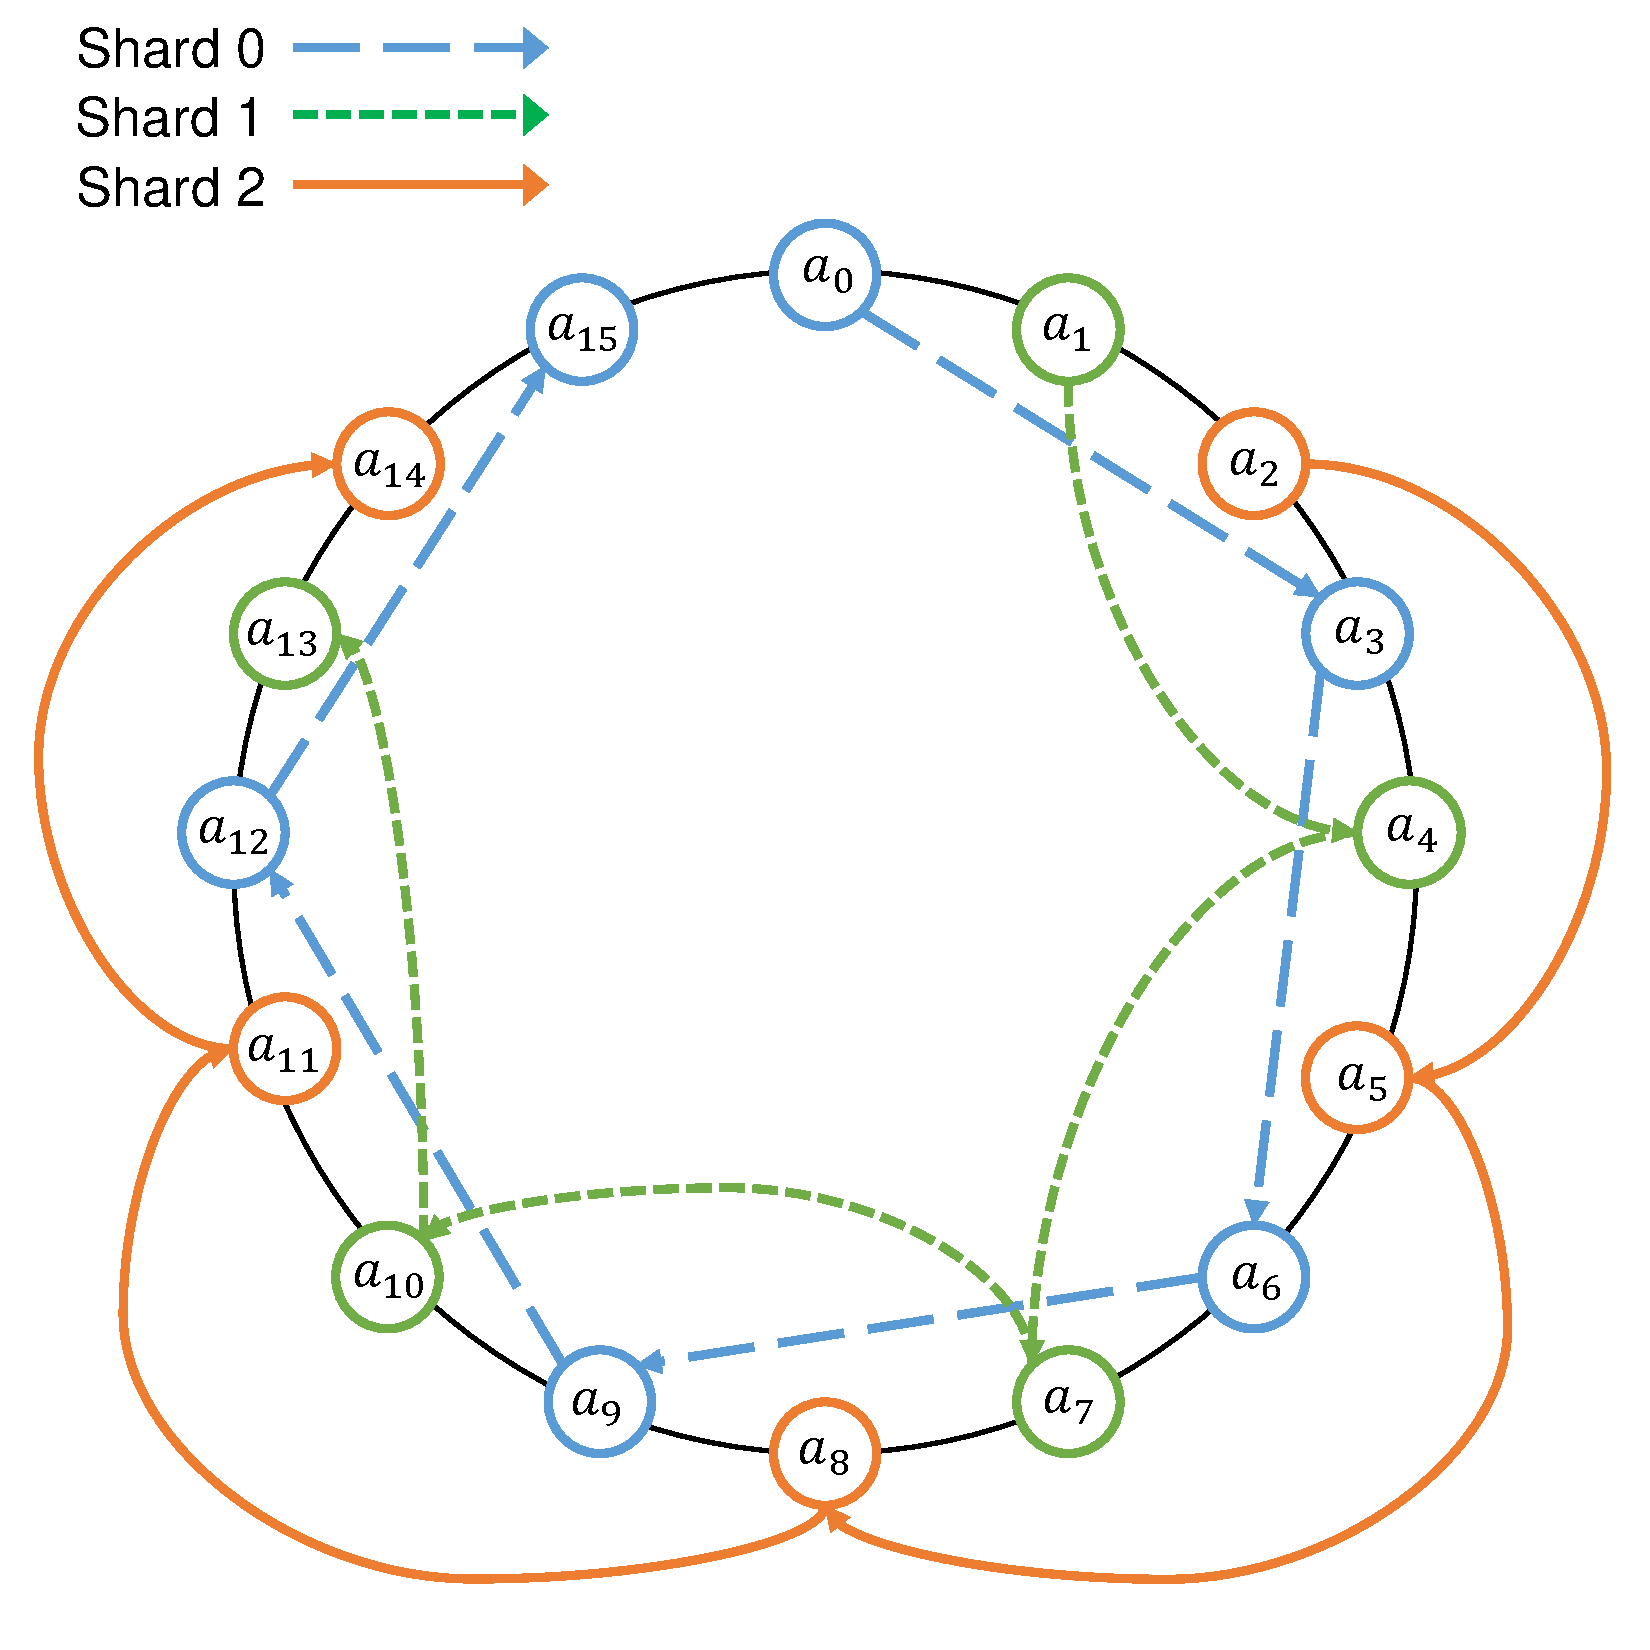
\includegraphics[width=\linewidth]{\ZippyFigures/shard_diagram.pdf}
\caption{\textbf{Sharding Visualization}\,---\,%
This is a configuration with three shards ($n = 3$). Shards $0,1,2$ are
initialized with starting addresses $a_0,a_1,a_2$. Each arrow represents
performing $a_i \cdot g^3$, a step forward by three elements in the
permutation.
}
\label{fig:sharding}
\end{figure}

\paragraph{Benchmarks}
To measure the impact of sharding in isolation from our other enhancements,
we conducted a series of scans, each covering a 1\% sample of the IP address
space, using our local blacklist file and a 10\,GigE uplink. Without
sharding, the average bandwidth utilization over 10~scans was 1.07 Gbps; with
sharding, the average increased to 1.80 Gbps, an improvement of 68\%.

\subsection{Blacklisting and Whitelisting}
 
ZMap address constraints are used to limit scans to specific areas of the
network (whitelisting) or to exclude particular address ranges
(blacklisting), such as IANA reserved allocations~\cite{iana}. Blacklisting
can also be used to comply with requests from network operators who want to
be excluded from receiving probe traffic. Good Internet citizenship demands
that ZMap users honor such requests, but after many scans over a prolonged
time period, a user's blacklist might contain hundreds of excluded prefixes.
 
Even with complicated address constraints, ZMap must be able to efficiently
determine whether any given IP address should be part of the scan. To support
10\,GigE linespeed, we implemented a combination tree- and array-based data
structure that can efficiently manipulate and query allowed addresses.

The IPv4 address space is modeled as a binary tree, where each node
corresponds to a network prefix. For example, the root represents 0.0.0.0/0,
and its children, if present, represent 0.0.0.0/1 and 128.0.0.0/1. Each
\emph{leaf} is colored either white or black, depending on whether or not the
corresponding prefix is allowed to be scanned. ZMap constructs the tree by
sequentially processing whitelist and blacklist entries that specify CIDR
prefixes. For each prefix, ZMap sets the color of the corresponding leaf,
adding new nodes or pruning the tree as necessary.

Querying whether an address may be scanned involves walking the tree,
beginning with the most significant bit of the address, until arriving at a
leaf and returning the color. However, a slightly different operation is used
during scanning. To make efficient use of the pseudorandom permutation
described above, we determine the number of allowed addresses $n$ (which may
be much smaller than the address space if a small whitelist is specified) and
select a permutation of approximately the same size. We then map from this
permutation of $1,\ldots,n$ to allowed addresses $a_1,\ldots,a_n$. Each node
in the tree maintains the total number of allowed addresses covered by its
descendants, allowing us to efficiently find the $i$th allowed address using
a simple recursive procedure.
%The ability to find specific addresses allows ZMap to utilize smaller cyclic
%groups to iterate over a small number of disjoint regions of address instead
%of iterating over the entire address space.\looseness=-1
 
As a further optimization, after the tree is constructed, we assemble a list
of /20 prefixes that are entirely allowed and reassign the address indices so
that these prefixes are ordered before any other allowed addresses. We then
use an array of these prefixes to optimize address lookups. If there are $m$
/20 prefixes that are allowed, then the first $m\cdot2^{12}$ allowed
addresses can be returned using only an array lookup, without needing to
consult the tree. The /20 size was determined empirically as a trade off
between lookup speed and memory usage.
 
\subsection{Zero-Copy NIC Access}
\label{sec:zc}
 
Despite ZMap's use of raw Ethernet sockets, sending each probe packet is an
expensive operation, as it involves a context switch for the \texttt{sendto}
system call and requires the scan packet to be transferred through kernel
space to the NIC~\cite{pfring-original, ten-gig-commodity}. Even with our
other enhancements, the high cost of these in-kernel operations prevented
ZMap from reaching above 2\,Gbps. To reduce these costs, we reimplemented
ZMap's network functionality using the PF\_RING ZC
interface~\cite{pfring-zc}. PF\_RING ZC allows userspace code to bypass the
kernel and have direct ``zero-copy'' access to the NIC\@, making it possible
to send packets without any context switches or wasted memory bandwidth.
 
To boost ZMap to 10\,GigE speeds, we implemented a new probe transmission
architecture on top of PF\_RING\@. This new architecture uses multiple
\emph{packet creation} threads that feed into a single \emph{send} thread. We
found that using more than one send thread for PF\_RING decreased the
performance of ZMap, but that a single packet creation thread was not fast
enough to reach line speed. By decoupling packet creation from sending, we
are able to combine the parallelization benefits of sharding with the speed
of PF\_RING\@.

In the original version of ZMap, multiple send threads each generated and
sent packets via a thread-specific raw Ethernet socket. We modify thread
responsibilities such that each packet creation thread iterates over one
address generation shard and generates and queues the packets. In a tight
loop, each packet generation loop calculates the next index in the shard,
finds the corresponding allowed IP address using the address constraint tree,
and creates an addressed packet in the PF\_RING ZC driver's memory. The
packet is added to a per-thread single-producer, single-consumer packet
queue. The send thread reads from each packet queue as packets come
available, and sends them over the wire using PF\_RING\@.

To determine the optimal number of packet creation threads, we performed a
series of tests, scanning for 50 seconds using 1--6 packet creation threads,
and measured the send rate. We find the optimal number of threads corresponds
with assigning one per physical core.
% Our results are show in Figure~\ref{fig:threads}.

\if0
\begin{figure}\centering
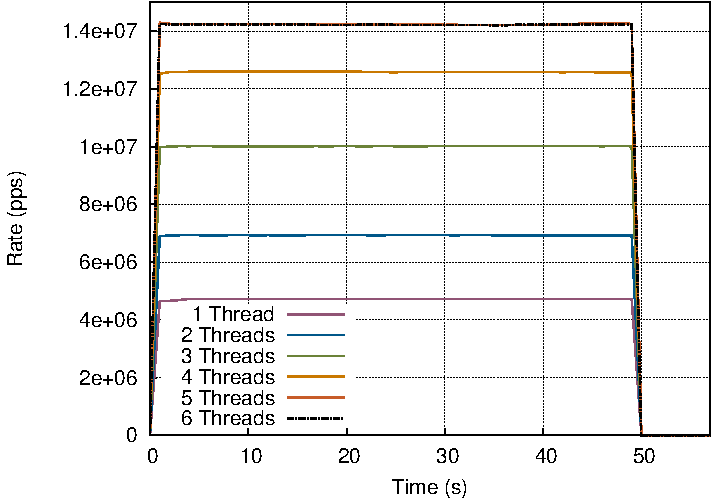
\includegraphics[width=\linewidth]{threads_vs_send.pdf}
\caption{\textbf{Threads vs.\ Scan Rate}\,---\,%
The send rate scales with the number of threads until reaching five threads,
at which point one thread is assigned per physical CPU. As threads begin to
share the same CPU, the send rate peaks. Using six threads results in an
identical send rate to five threads.
}
\label{fig:threads}
\end{figure}
\fi

\if0
\paragraph{Benchmarks}
We compared zero-copy NIC access to ZMap's traditional packet sending
architecture. In each case we also enabled the enhancements discussed in
Section~\ref{sec:TK} and Section~\ref{sec:TK} and conducted repeated scans of
covering 2\% samples of the public IPv4 address space. The average
transmission rate improved from 2.6~Mpps to 14.23~Mpps, a 447\% improvement.
This is 96\% of the theoretical limit of 10\,GigE,
14.88~Mpps~\cite{ten-gig-commodity}.
\fi

\begin{table}\centering
    \begin{tabular}{lrr}
    \toprule
    \textbf{Scan Rate} & \textbf{Hit Rate} & \textbf{Duration} \\ \midrule
    1.44 Mpps ($\approx$1\,GigE)                 & 1.00  & 42:08               \\ 
    3.00 Mpps                  & 0.99  & 20:47              \\ 
    4.00 Mpps                  & 0.97  & 15:38              \\
    14.23 Mpps ($\approx$10\,GigE)                 &  0.63 &  4:29               \\ % raw is 0.675
    \bottomrule
    \end{tabular}
    % 0.675
\caption{\textbf{Performance of Internet-wide Scans}\,---\,%
We show the scan rate, the normalized hit rate, and the scan duration (m:s)
for complete Internet-wide scans performed with optimized ZMap.}
\label{tbl:fullhitrate}
\end{table}

\section{Evaluation}
\label{sec:evaluation}

We performed a series of experiments to characterize the behavior of scanning
at speeds greater than 1~Gbps. In our test setup, we completed a full scan of
the public IPv4 address space in 4m29s on a server with a 10\,GigE uplink.
However, at full speed the number of scan results (the hit rate) decreased by
37\% compared to a scan at 1~Gbps, due to random packet drop. We find that we
can scan at speeds of up to 2.7~Gbps before seeing a substantial drop in hit
rate.

We performed the following measurements on a Dell PowerEdge R720 with two
Intel Xeon E5-2690 2.9~GHz processors (8 physical cores each plus
hyper-threading) and 128~GB of memory running Ubuntu 12.04.4~LTS and the
3.2.0-59-generic Linux kernel. We use a single port on a Intel X540-AT2
(rev~01) 10\,GigE controller as our scan interface, using the PF\_RING-aware
\texttt{ixgbe} driver bundled with PF\_RING 6.0.1. We configured ZMap to use
one send thread, one receive thread, one monitor thread, and five packet
creation threads.

We used a 10\,GigE network connection at the University of Michigan Computer
Science and Engineering division connected directly to the building uplink,
an aggregated $2\times 10$\,GigE channel. Beyond the 10\,GigE connection, the
only special network configuration arranged was static IP addresses. We note
that ZMap's performance may be different on other networks depending on local
congestion and upstream network conditions.\looseness=1

We performed all of our experiments using our local blacklist file. Our
blacklist, which eliminates non-routable address space and networks that have
requested exclusion from scanning~\cite{state-of-scanning}, consists of over
1,000 entries of various-sized network blocks. It results in 3.7~billion
allowed addresses---with almost all the excluded space consisting of IANA
reserved allocations.

\subsection{Hit-rate vs.\ Scan-rate}

In our original ZMap study, we experimented with various scanning speeds up
to gigabit Ethernet line speed (1.44~Mpps) and found no significant effect on
the number of results ZMap found~\cite{zmap}. In other words, from our
network, ZMap did not appear to miss any results when it ran faster up to
gigabit speed.

In order to determine whether hit-rate decreases with speeds higher than
1~Gigabit, we performed 50~second scans at speeds ranging from 0.1--14~Mpps.
We performed 3~trials at each scan rate. As can be seen in
Figure~\ref{fig:hitrate}, hit-rate begins to drop linearly after 4~Mpps. At
14~Mpps (close to 10\,GigE linespeed), the hit rate is 68\% of the hit rate
for a 1\,GigE scan. However, it is not immediately clear why this packet drop
is occurring at these higher speeds---are probe packets dropped by the
network, responses dropped by the network, or packets dropped on the scan
host due to ZMap?

\begin{figure}[t]\centering
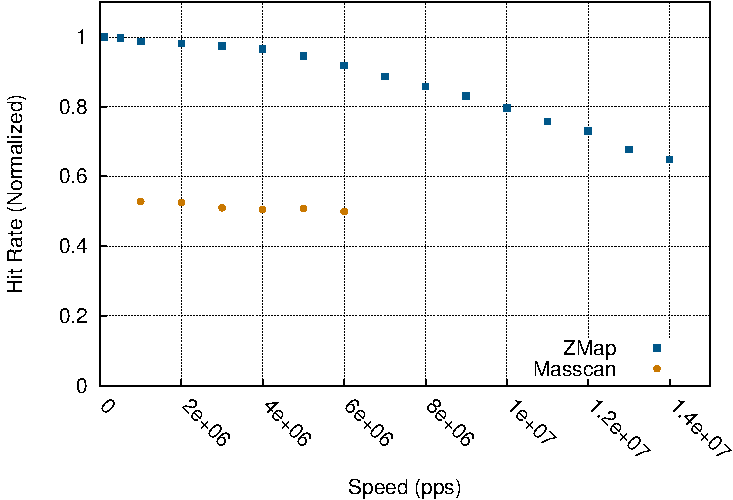
\includegraphics[height=2.1in]{\ZippyFigures/norm_avg_hitrate.pdf}
\caption{\textbf{Hit-rate vs.\ Scan-rate}\,---\,%
ZMap's hit rate is roughly stable up to a scan rate of 4~Mpps, then declines
linearly. This drop off may be due to upstreudegrm network congestion. Even using
PF\_RING, Masscan is unable to achieve scan rates above 6.4~Mpps on the same
hardware and has a much lower hit rate.}
\label{fig:hitrate}
\end{figure}

\begin{figure}[t]\centering
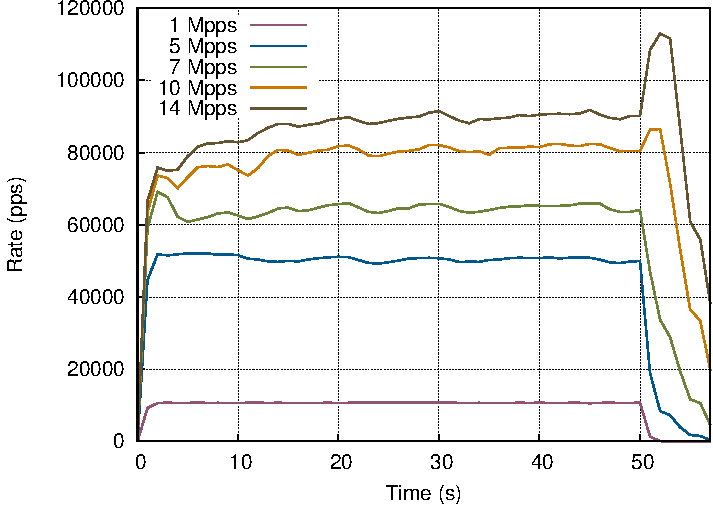
\includegraphics[height=2.1in]{\ZippyFigures/avg_count_recv_succs.pdf}
\caption{\textbf{Response Rate During Scans}\,---\,%
This graph shows the rate of incoming SYN-ACKs during 50-second scans. The
peaks at the end (after sending finishes) at rates above 7~Mpps indicate that
many responses are being dropped and retransmitted before being recorded by
ZMap.}
\label{fig:recvrate}
\end{figure}

We first investigate whether response packets are being dropped by ZMap or
the network. In the original ZMap work, we found that 99\% of hosts respond
within 1~second~\cite{zmap}. As such, we would expect that after 1~second,
there would be negligible responses. However, as can be seen in
Figure~\ref{fig:recvrate}, there is an unexpected spike in response packets
after sending completes at 50~seconds for scans at 10 and 14~Mpps. This spike
likely indicates that response packets are being dropped by our network, NIC,
or ZMap, as destination hosts will resend SYN-ACK packets for more than one
minute if an ACK or RST packet is not received.

In order to determine whether the drop of response packets is due to ZMap
inefficiencies or upstream network congestion, we performed a secondary scan
in which we split the probe generation and address processing onto separate
machines. The send machine remained the same. The receive machine was an HP
ProLiant DL120 G7, with an Intel Xeon E3-1230 processor (4 cores with
hyperthreading) and 16~GB of memory, running Ubuntu 12.04.4~LTS and the
3.5.0-52-generic Linux kernel.

As we show in Figure~\ref{fig:twomachines}, this spike does not occur when
processing response packets on a secondary server---instead it closely
follows the pattern of the slower scans. This indicates that ZMap is locally
dropping response packets. However, the split setup received only 4.3\% more
packets than the single machine---not enough to account for the 31.7\%
difference between a 14~Mpps and a 1~Mpps scan. If a large number of response
packets were dropped due to network congestion, we would not have observed an
immediate drop in responses---likely indicating that the root cause of the
decreased hit-rate is dropped probe packets.

It is not immediately clear where probe packets are dropped---it is possible
that packets are dropped locally by PF\_RING, are dropped by local routers
due to congestion, or that we are overwhelming destination networks. PF\_RING
records locally dropped packets, which remained zero throughout our scans,
which indicates that packets are not being dropped locally. In order to
locate where packet drop is occurring on our network, we calculated the drop
rate per AS and found little AS-level correlation for packets dropped by the
10\,GigE scans, which suggests that random packet drop is occurring close to
our network rather than at particular distant destination networks.

\begin{figure}\centering
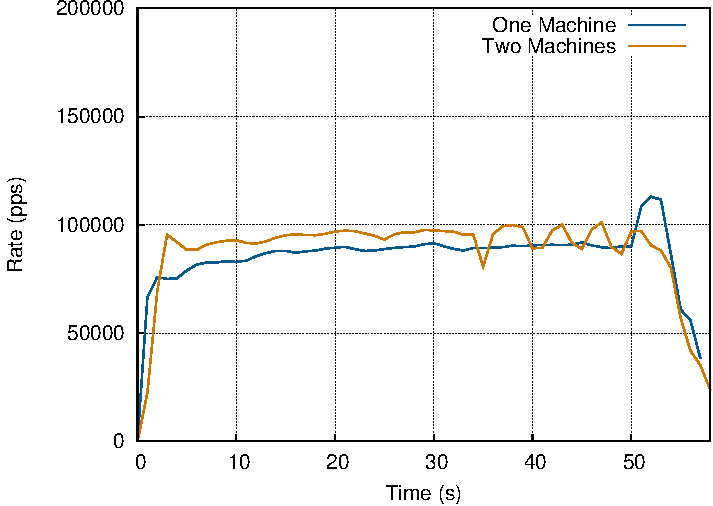
\includegraphics[width=\linewidth]{\ZippyFigures/split_avg_count_recv_succs.pdf}
\caption{\textbf{Comparing One and Two Machines}\,---\,%
If we scan at 14~Mpps and use separate machines for the sending and receiving
tasks, the spike in the SYN-ACK rate at 50~s disappears, indicating that
fewer packets are dropped with the workload spread over two machines.
However, overall the two machine configuration received only 4.3\% more
responses than with one machine, which suggests that network packet loss
accounts for the majority of the drop off at higher scan rates.}
\label{fig:twomachines}
\end{figure}

\subsection{Complete Scans}

We completed a full Internet-wide scan, allowing ZMap to operate at its full
scan rate. This scan achieved an average 14.23~Mpps---96\% of the theoretical
limit of 10\,GigE, completing in 4~minutes, 29~seconds and achieving a hit
rate that is 62.5\% of that from a 1\,GigE scan. We show a comparison to
lower speed scans in Table~\ref{tbl:fullhitrate}. As we discussed in the
previous section, this decrease is likely due to local network congestion,
which results in dropped probe packets. However, more investigation is
deserved in order to understand the full dynamics of high-speed scans.

\subsection{Comparison to Masscan}
\label{sec:masscan-comparison}

\begin{figure*}\centering
\hfill
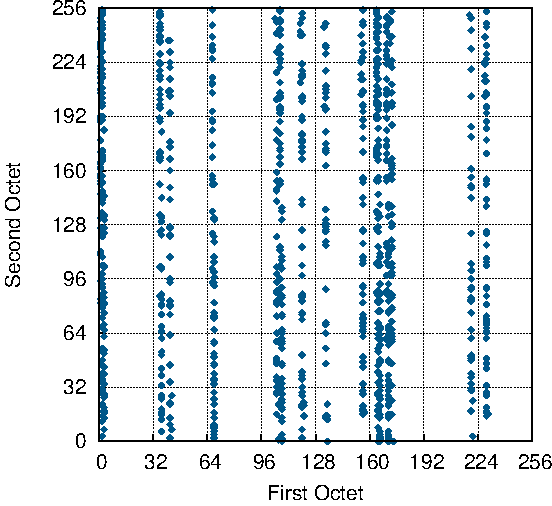
\includegraphics[height=2.5in]{\ZippyFigures/masscan_randomness.pdf}
\hfill\hfill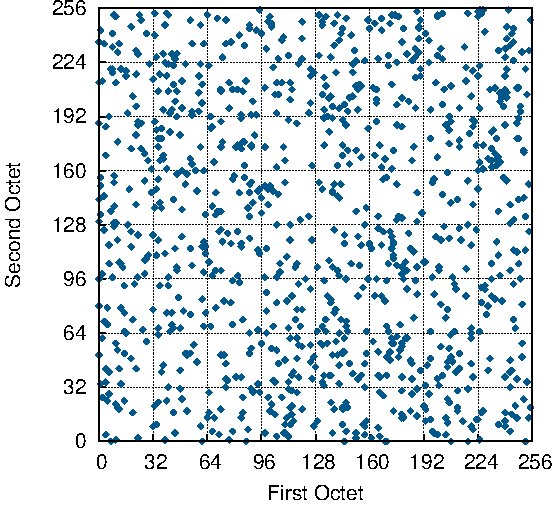
\includegraphics[height=2.5in]{\ZippyFigures/zmap_randomness.pdf}
\hfill\strut
\caption{\textbf{Address Randomization Comparison}\,---\,%
These plots depict the first 1000 addresses of an Internet-wide scan selected
by Masscan (\emph{left}) and ZMap (\emph{right}), with the first and second
octets mapped to the $x$ and~$y$ coordinates. ZMap's address randomization is
CPU intensive but achieves better statistical properties than the cheaper
approach used by Masscan, enabling valid sampling. We enhanced ZMap to
distribute address generation across multiple cores.}
\label{fig:randomy}
\end{figure*}

Masscan advertises the ability to emit probes at 25~Mpps using PF\_RING and
two 10\,GigE adapters, each configured with two RSS queues---84\% of
linespeed for dual 10\,GigE and 166\% of linespeed for a single 10\,GigE
adapter~\cite{masscan-10g}. We benchmarked ZMap and Masscan using the
Xeon~E3-1230 machine described above. In our experiments, we found that
Masscan was able to send at a peak 7.4~Mpps using a single-adapter
configuration with two RSS queues, 50\% of 10\,GigE linespeed. On the same
hardware, ZMap is capable of reaching a peak 14.1~Mpps. While Masscan may be
able to achieve a higher maximum speed using multiple adapters, ZMap is able
to fully saturate a 10\,GigE uplink with a single adapter.

Masscan uses a custom Feistel network to ``encrypt'' a monotonically
increasing index to generate a random permutation of the IPv4 address
space~\cite{masscan-rng}. While this is computation cheaper than using a
cyclic group, this technique results in poor statistical properties, which we
show in Figure~\ref{fig:randomy}. This has two consequences: first, it is not
suitable for sampling portions of the address space, and second, there is
greater potential for overloading destination networks. This could explain
the discrepency in Figure~\ref{fig:hitrate} if Masscan targeted a less
populated subnet.

Masscan and ZMap use a similar sharding approach to parallelize address
generation and distribute scans. Both programs ``count off'' addresses into
shards by staggering the offsets of the starting position of each shard
within the permutation and iterating a fixed number of steps through each of
their permutations. In ZMap, this is implemented by replacing the iteration
factor $g$ with $g^n$. In Masscan, this is simply a matter of incrementing
the monotonically increasing index by more than one.


\section{Applications}
\label{sec:discussion}

In this section, we consider applications that could benefit from 10\,GigE
scanning and remark on the implications of high-speed scanning for defenders
and attackers.

Scanning at faster rates reduces the blur introduced from hosts changing IP
addresses by decreasing the number of hosts that may be doubly counted during
longer scans. This also increases the ability to discover hosts that are only
online briefly. Thus, the ability to complete scans in minutes allows
researchers to more accurately create a snapshot of the Internet at a given
moment.

Similarly, the increased scan rate enables researchers to complete
high-resolution scans when measuring temporal effects. For example, while
researchers were able to complete comprehensive scans for the recent
Heartbleed Vulnerability every few hours~\cite{zmap-heartbleed}, many sites
were patched within the first minutes after disclosure. The ability to scan
more rapidly could help shed light on patching behavior within this critical
initial period.

\begin{figure*}
\centering
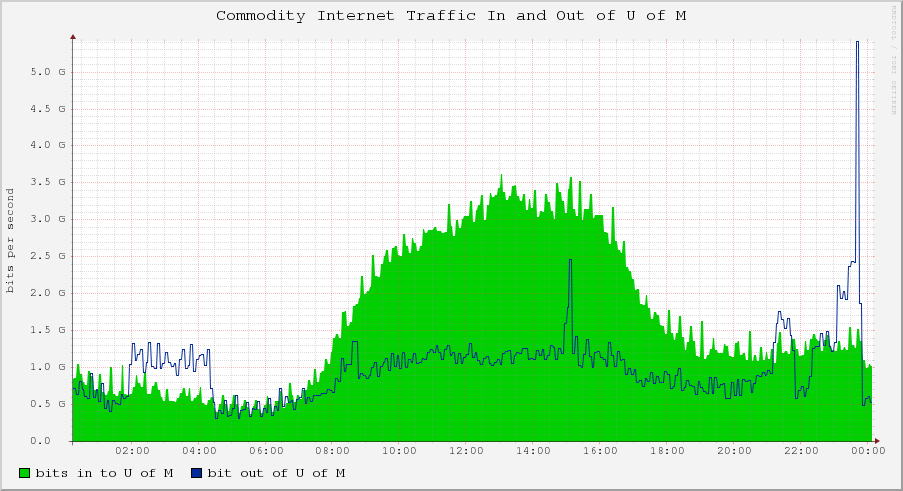
\includegraphics[width=0.75\linewidth]{\ZippyFigures/graph_image.png}
\caption{\textbf{10\,GigE   Scan Traffic}\,---\,%
An Internet-wide scan at full 10\,GigE speed dwarfed all other traffic at the
university during this 24~hour period. At 14.23~Mpps, a single machine
running ZMap generated 4.6~Gbps in outgoing IP traffic and scanned the entire
public IPv4 address space in 4m29s. The massive increase in outbound traffic
appears to have caused elevated packet drop. Notable smaller spikes are due
to earlier experiments.}
\label{fig:traffic}
\end{figure*}

Faster scan rates also allow for a variety of new scanning-related
applications that require multiple packets, including quickly completing
global trace routes or performing operating system fingerprinting.
Furthermore, the advancement of single-port scanning can be utilized to
quickly perform scans of a large number of ports, allowing scanning all
privileged ports on a /16 in under 5~seconds and \emph{all} ports in
5~minutes, assuming the attacker has sufficient bandwidth to the target.

The most alarming malicious potential for 10\,GigE scanning lies in its
ability to find and exploit vulnerabilities \emph{en masse} in a very short
time. Durumeric et~al.\ found that attackers began scanning for the
Heartbleed vulnerability within 22~hours of its
disclosure~\cite{zmap-heartbleed}. While attackers have utilized botnets and
worms in order to complete distributed scans for vulnerabilities, recent
work~\cite{state-of-scanning} has shown that attackers are now also using
ZMap, Masscan, and other scanning technology from bullet-proof hosting
providers in order to find vulnerable hosts. The increase in scan rates could
allow attackers to complete Internet-wide vulnerability scans in minutes as
10\,GigE becomes widely available.\looseness=-1

\section{Future Work}

We demonstrated that it is possible to perform Internet-wide scans at
10\,GigE linespeed, but, at least from our institutional network, we are
unable to sustain the expected hit rate as scanning approaches this packet
rate. Further investigation is needed to understand this effect and profile
ZMap's performance on other networks. One important question is whether the
drop off is caused by nearby network bottlenecks (which might be reduced with
upgraded network hardware) or whether it arises because such rapid scanning
induces congestion on many distant networks---which would represent an
inherent limit on scan speed. It is also possible that there are a small
number of remote bottlenecks that cause the observed drop in hit rate at high
speeds. In that case, identifying, profiling, and removing these bottlenecks
could improve performance.

40\,GigE hardware currently exists, and 100\,GigE is under
development~\cite{hundred-gig}. As these networks become more widely
available, it may be desirable to optimize and scale Internet-wide scanning
to even higher speeds.

\section{Conclusion}

In this work, we introduced enhancements to the ZMap Internet scanner that
enable it to scan at up to 14.2~Mpps. The three modifications we
present---sharding, optimized address constraints, and integration with
PF\_RING ZC---enable scanning at close to 10\,GigE linespeed. These
modifications are available now on experimental ZMap branches and will be
merged into mainline ZMap.

With these enhancements, we are able to complete a scan of the public IPv4
address space in 4m29s. However, despite having a well provisioned upstream
network, coverage in our experiments drops precipitously when scanning faster
than 4~Mpps. While further research is needed to better characterize and
reduce the causes of this drop off, it may be related to specific conditions
on our network.

As faster network infrastructure becomes more widely available, 10\,GigE
scanning will enable powerful new applications for both researchers and
attackers.

\section*{Acknowledgments}

The authors thank the exceptional sysadmins at the University of Michigan for
their help and support throughout this project. This research would not have
been possible without Kevin Cheek, Chris Brenner, Laura Fink, Paul Howell,
Don Winsor, and others from ITS, CAEN, and DCO\@. We are grateful to Michael
Bailey for numerous productive discussions, to Luca Deri and ntop for
providing a PF\_RING license, and to the many contributors to the ZMap open
source project. We also thank Denis Bueno, Jakub Czyz, Henry Fanson, Pat
Pannuto, and Eric Wustrow.

This material is based upon work supported by the National Science Foundation
under Grant No.~CNS-1255153 and No.~CNS-0964545. Any opinions, findings, and
conclusions or recommendations expressed in this material are those of the
authors and do not necessarily reflect the views of the National Science
Foundation.

%% !TEX root = ../../../proposal.tex

{\footnotesize\bibliographystyle{abbrv}
\balance
\bibliography{woot}}
\end{document}



\chapter{Logjam}
%% !TEX root = ../../../proposal.tex

\newcommand*{\ZippyPaper}{papers/zippy/paper}
\newcommand*{\ZippyFigures}{papers/zippy/figures}
%% !TEX root = ../../../proposal.tex

\documentclass[letterpaper,twocolumn,10pt]{article}
\usepackage{usenix,epsfig,footnote,url}\urlstyle{rm}
\usepackage[T1]{fontenc}
\usepackage[%
    breaklinks=true,colorlinks=true,linkcolor=black,%
     citecolor=black,urlcolor=black,bookmarks=true,bookmarksopen=false,%
    pdfauthor={David Adrian, Zakir Durumeric, Gulshan Singh, and J. Alex Halderman},
    pdftitle={Zippier ZMap: Internet-Wide Scanning at 10 Gbps}
    ,pdftex]{hyperref}
\usepackage{amsmath, amssymb, amsfonts, amsthm}
\usepackage{mathptmx}\renewcommand{\ttdefault}{cmtt}
\usepackage[margin=0pt,font=small]{caption}
\usepackage{graphicx}
\usepackage{booktabs}
\usepackage{balance}
\usepackage{cite}
\usepackage[protrusion=true,expansion=true,kerning]{microtype}
\SetExtraKerning % Add space around emdashes
   { encoding = *,
        font = * }
   { \textemdash  = {120,120} }

% Fix ugly USENIX subsection headings (AH 3/08)
\makeatletter
\renewcommand{\section}{\@startsection {section}{1}{\z@}%
                                   {-3.5ex plus-1ex minus -.2ex}%
                                   {2.3ex plus.2ex}%
                                   {\normalfont\large\bfseries}}
\renewcommand{\subsection}{\@startsection{subsection}{2}{\z@}%
                                     {-2.5ex plus-.7ex minus -.2ex}%
                                     {1.5ex plus .2ex}%
                                     {\normalfont\fontsize{11}{12.5}\bfseries}}
\makeatother

% Paragraph and subpar
\renewcommand{\paragraph}[1]{\medskip\noindent\textbf{#1}\quad}
\newcommand{\subpar}[1]{\medskip\noindent\textsl{#1}\enspace}

% Stop URLs from hyphenating after  "http:" (AH 12/08)
\def\UrlBreaks{\do-\do\.\do\@\do\\\do\!\do\_\do\|\do\;\do\>\do\]%
 \do\)\do\,\do\?\do\'\do+\do\=\do\#}
\def\UrlBigBreaks{\do\:\do\/}%

% TODO, TK, etc. (AH 4/12)
\usepackage{xspace}
\newcommand{\todo}[1]{{\color{red}{\textbf{\em [TODO: #1]}}}\xspace}
\newcommand{\TODO}[1]{\todo{#1}}
\newcommand{\tk}{{\color{red}{\bf TK}}\xspace}
\newcommand{\TK}{\tk}
\newcommand{\comment}[1]{\relax} % comment out text
\newcommand{\xcite}[1]{\relax} % comment out citation

\newif\ifweb\webtrue
\ifweb
    \usepackage{watermark}
    \thiswatermark{\parbox{\textwidth}{\vskip30pt\centering
    \vspace*{-20pt}%
     This paper appeared in \emph{Proceedings of the 8th {USENIX} Workshop on Offensive Technologies} (WOOT '14), August~2014.\\
    \vskip6pt
    \rule[\baselineskip]{\textwidth}{0.5pt}
    }}
\fi

\begin{document}
\pagenumbering{arabic}
\thispagestyle{empty}

% Some math stuff
\newcommand{\bbZ}{\mathbb{Z}}

%don't want date printed
\date{}

\title{\Large\bf Zippier ZMap: Internet-Wide Scanning at 10\,Gbps}

\author{
{\rm David Adrian, Zakir Durumeric, Gulshan Singh, and J.\,Alex Halderman}\smallskip\\
University of Michigan\\
\small\rm\{davadria,\,zakir,\,gulshan,\,jhalderm\}@umich.edu
}
 

\maketitle


\begin{abstract}
We introduce optimizations to the ZMap network scanner that achieve a 10-fold
increase in maximum scan rate. By parallelizing address generation,
introducing an improved blacklisting algorithm, and using zero-copy NIC
access, we drive ZMap to nearly the maximum throughput of
10~gigabit~Ethernet, almost 15 million probes per second. With these changes,
ZMap can comprehensively scan for a single TCP port across the entire public
IPv4 address space in 4.5~minutes given adequate upstream bandwidth. We
consider the implications of such rapid scanning for both defenders and
attackers, and we briefly discuss a range of potential
applications.\looseness=1
\end{abstract}

\section{Introduction}
\label{sec:introduction}

In August 2013, we released ZMap, an open-source network scanner designed to
quickly perform Internet-wide network surveys~\cite{zmap}. From a single
machine, ZMap is capable of scanning at 1.44~million packets per second
(Mpps), the theoretical limit of gigabit Ethernet. At this speed, ZMap can
complete a scan targeting one TCP port across the entire public IPv4 address
space in under 45~minutes---a dramatic improvement compared to
weeks~\cite{zmap} or months~\cite{sslobservatory} required using Nmap. Yet
even at gigabit linespeed, ZMap does not utilize the full bandwidth of the
fastest readily available connections: 10\,GigE uplinks are now offered by
Amazon~EC2~\cite{amazon-10g} and at a growing number of research
institutions. \looseness=-1

In this paper, we scale ZMap to 10\,GigE speeds by introducing a series of
performance enhancements. These optimizations allow scanning speeds that
provide higher temporal resolution when conducting Internet-wide surveys and
make it possible to quickly complete complex multipacket studies.

Scanning at 10\,GigE linespeed necessitates sending nearly 15~Mpps
continuously. For single-packet probes such as SYN scans, this allows only
200 cycles per probe on a 3\,GHz core. An L2 cache miss might incur a cost of
almost 100 cycles, so it essential to make efficient use of both CPU and
memory. In order to generate and transmit packets at this rate, we introduce
modifications that target the three most expensive per-probe operations in
ZMap:
\begin{enumerate}
  \item \emph{Parallelized address generation.}\quad
    ZMap uses a multiplicative cyclic group to iterate over a random permutation
    of the address space, but this becomes a bottleneck at multigigabit speeds.
    We implement a mutex-free sharding mechanism that spreads address generation
    across multiple threads and cores.
  \item \emph{Optimized address constraints.}\quad
    Responsible scanning requires honoring requests from networks that opt out,
    but over time this can result in large and complex blacklists. We develop an
    optimized address constraint data structure that allows ZMap to efficiently
    cycle through allowed targets.
  \item \emph{Zero-copy packet transmission.}\quad
    ZMap sends Ethernet frames using a raw socket, which avoids the kernel's
    TCP/IP stack but still incurs a per-packet context switch. We switch to using
    the PF\_RING Zero Copy (ZC) interface, which bypasses the kernel and reduces
    memory bandwidth.
\end{enumerate}

These enhancements enable ZMap to scan at 14.23~Mpps, 96\% of the theoretical
limit of 10\,GigE\@. In order to confirm these performance gains, we
completed a full scan of the IPv4 address space in 4m29s---to our knowledge,
the fastest Internet-wide scan yet reported.

The ability to scan at 10\,GigE speeds creates new opportunities for security
researchers. It allows for truer snapshots of the state of the Internet by
reducing error due to hosts that move or change during the scan. Likewise, it
enables more accurate measurement of time-critical phenomena, such as
vulnerability patching in the minutes and hours after public disclosure. On
the other hand, it raises the possibility that attackers could use 10\,GigE
to exploit vulnerabilities with alarming speed.

\section{Related Work}
\label{sec:relatedwork}

Many network scanning tools have been
introduced~\cite{scanrand,unicornscan,masscan-10g,nmap,zmap}, although until
recently most were designed for scanning small networks. One of the most
popular is Nmap~\cite{nmap}, a highly capable network exploration tool. Nmap
is well suited for vertical scans of small networks or individual hosts, but
the original ZMap implementation outperformed it on horizontal Internet-wide
scans by a factor of 1300~\cite{zmap}. Our enhancements to ZMap improve its
performance by another factor of ten.

ZMap is not the first Internet-wide scanner to use PF\_RING to send at speeds
greater than 1~Gbps. Masscan, released in September 2013, also utilizes
PF\_RING and claims the ability to scan at 25~Mpps using dual 10\,GigE
ports---84\% of the theoretical limit of dual 10\,GigE~\cite{masscan-10g}. We
present a more detailed comparison to Masscan in
Section~\ref{sec:masscan-comparison}. While the Masscan team did not have the
facilities to perform live network tests at rates higher than
100,000~pps~\cite{masscan-10g}, we report what we believe is the first
Internet-wide scan conducted at 10\,GigE speeds.

\section{Performance Optimizations}
\label{sec:optimizations}

ZMap achieves this performance based on a series of architectural choices
that are geared towards very large, high-speed scans~\cite{zmap}. It avoids
per-connection state by embedding tracking information in packet fields that
will be echoed by the remote host, using an approach similar to
SYN~cookies~\cite{bernstein1996syn}. It eschews timeouts and simplifies flow
control by scanning according to a random permutation of the address space.
Finally, it avoids the OS's TCP/IP stack and writes raw Ethernet frames.

This architecture allows ZMap to exceed gigabit Ethernet linespeed on
commodity hardware, but there are several bottlenecks that prevent it from
fully reaching 10\,GigE speeds. ZMap's address generation is CPU intensive
and requires a global lock, adding significant overhead. Blacklisting ranges
of addresses is expensive and scales poorly. Sending each packet requires a
context switch and unnecessary copies as packets are passed from userspace to
the kernel and then to the NIC~\cite{multi-core-network}. We implement
optimizations that reduce each of these bottlenecks.

\subsection{Address Generation Sharding}

Address generation in ZMap is designed to achieve two goals. First, it avoids
flooding destination networks by ordering targets according to a pseudorandom
permutation of the address space. Second, it enables statistically valid
sampling of the address space.
% by ensuring that prefixes of the permutation have good statistical
% randomness. However, on a per-probe basis, address generation is one of the
% most costly operations.

ZMap iterates over a multiplicative group of integers modulo $p$ that
represent 32-bit IPv4 addresses. By choosing $p$ to be $2^{32} + 15$, the
smallest prime larger than $2^{32}$, we guarantee that the group
$(\bbZ/p\bbZ)^{\times}$ is cyclic and that it covers the full IPv4 address
space. ZMap derives a new random primitive root $g$ for each scan in order to
generate new permutation of the address space. The scanner starts at a random
initial address $a_{0}$ and calculates $a_{i+1} = g \cdot a_{i} \bmod p$ to
iterate through the permutation. The iteration is complete when $a_{i+1}$
equals $a_{0}$.

The most expensive part of this scheme is the modulo operation, which must be
performed at every step of the iteration. Unfortunately, the modulo operation
cannot currently be performed by multiple threads at once, because each
address in the permutation is dependent on the previous---calculating the
next address requires acquiring a lock over the entire iterator state.

To remove this bottleneck and efficiently distribute address generation over
multiple cores, we extend ZMap to support sharding. In the context of ZMap, a
shard is a partition of the IPv4 address space that can be iterated over
independently from other shards; assigning one shard to each thread allows
for independent, mutex-free execution. Each shard contains a disjoint subset
of the group, with the union of all the shards covering the entire group.

To define $n$ shards, we choose an initial random address $a_0$ and assign
each sequential address $a_j$ in the permutation to shard $j \bmod n$. To
implement this, we initialize shards $1 \dots n$ with starting addresses
$a_0,\dots,a_{n-1}$, which can be efficiently calculated as $a_0 \cdot
g^{0,\dots,n-1}$. To iterate, we replace $g$ with $g^n$, which ``skips
forward'' in the permutation by $n$ elements at each step. Each shard
computes $a_{i+1} = a_i \cdot g^n \bmod p$ until reaching its shard specific
ending address $a_{e_j}$. For example, if there were three shards, the first
would scan
$\{ {a_0,\; a_3=g^3 \cdot a_0,\; a_6 = g^3 \cdot a_3,\dots,\; a_{e_1}} \}$,
second
$\{ {a_1,\; a_4=g^3 \cdot a_4,\; a_7 = g^3 \cdot a_4,\dots,\; a_{e_2}} \}$, 
and third 
$\{ {a_2,\; a_5=g^3 \cdot a_0,\; a_8 = g^3 \cdot a_5,\dots,\; a_{e_3}} \}$. 
We illustrate the process in Figure~\ref{fig:sharding}.

After pre-calculating the shard parameters, we only need to store three
integers per shard: the starting address $a_0$, the ending address $a_e$, and
the current address $a_i$. The iteration factor $g^n$ and modulus $p$ are the
same for all shards. Each thread can then iterate over a single shard
independently of the other threads, and no global lock is needed to determine
the next address to scan. Multiple shards can operate within the same ZMap
process as threads (the configuration we evaluate in this paper), or they can
be split across multiple machines in a distributed scanning mode.

\begin{figure}\centering
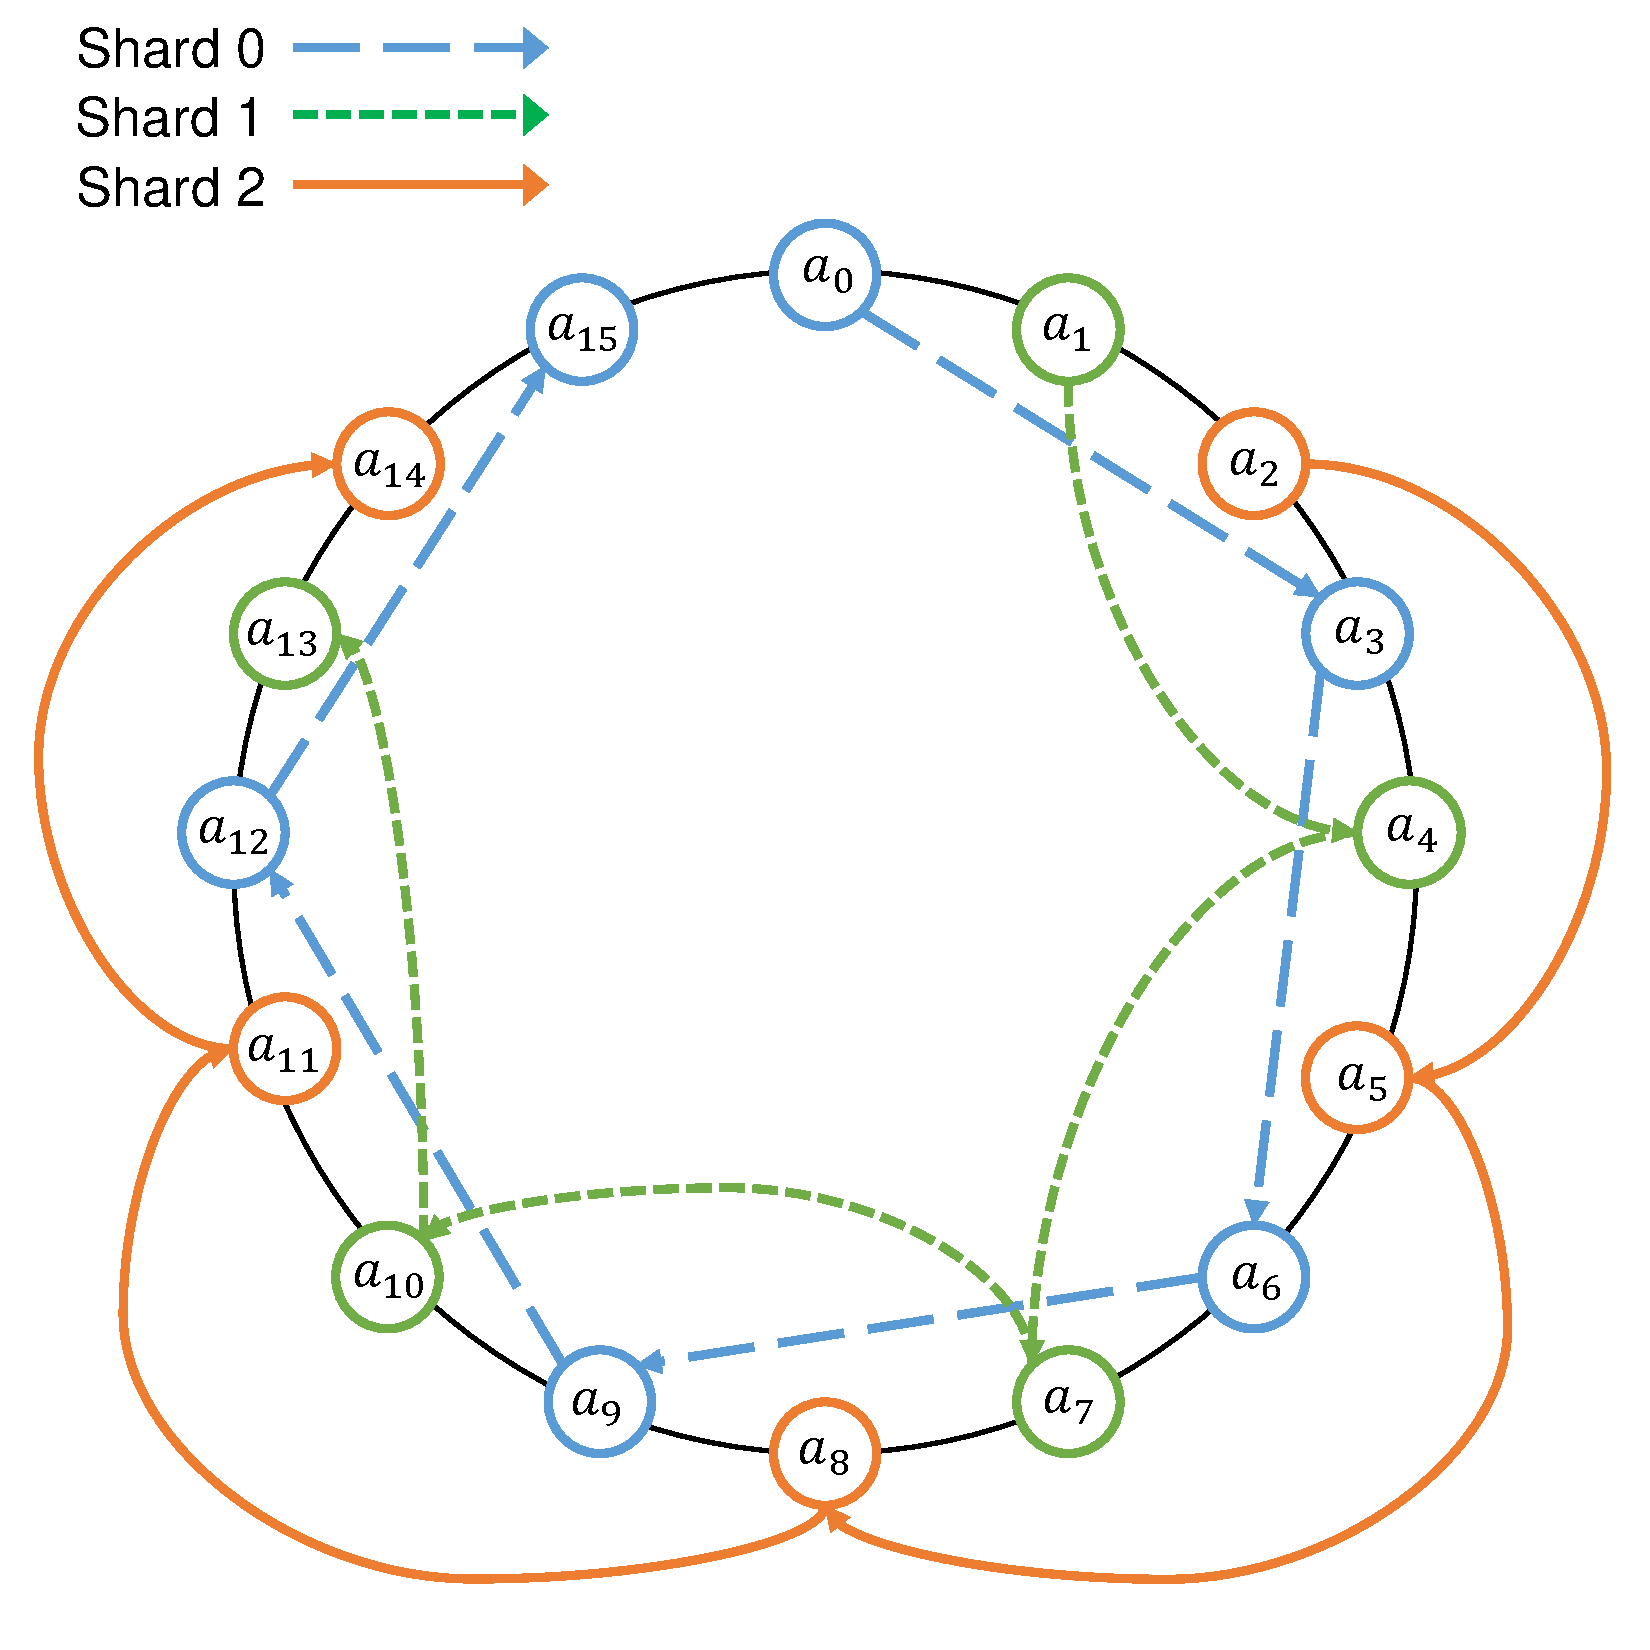
\includegraphics[width=\linewidth]{\ZippyFigures/shard_diagram.pdf}
\caption{\textbf{Sharding Visualization}\,---\,%
This is a configuration with three shards ($n = 3$). Shards $0,1,2$ are
initialized with starting addresses $a_0,a_1,a_2$. Each arrow represents
performing $a_i \cdot g^3$, a step forward by three elements in the
permutation.
}
\label{fig:sharding}
\end{figure}

\paragraph{Benchmarks}
To measure the impact of sharding in isolation from our other enhancements,
we conducted a series of scans, each covering a 1\% sample of the IP address
space, using our local blacklist file and a 10\,GigE uplink. Without
sharding, the average bandwidth utilization over 10~scans was 1.07 Gbps; with
sharding, the average increased to 1.80 Gbps, an improvement of 68\%.

\subsection{Blacklisting and Whitelisting}
 
ZMap address constraints are used to limit scans to specific areas of the
network (whitelisting) or to exclude particular address ranges
(blacklisting), such as IANA reserved allocations~\cite{iana}. Blacklisting
can also be used to comply with requests from network operators who want to
be excluded from receiving probe traffic. Good Internet citizenship demands
that ZMap users honor such requests, but after many scans over a prolonged
time period, a user's blacklist might contain hundreds of excluded prefixes.
 
Even with complicated address constraints, ZMap must be able to efficiently
determine whether any given IP address should be part of the scan. To support
10\,GigE linespeed, we implemented a combination tree- and array-based data
structure that can efficiently manipulate and query allowed addresses.

The IPv4 address space is modeled as a binary tree, where each node
corresponds to a network prefix. For example, the root represents 0.0.0.0/0,
and its children, if present, represent 0.0.0.0/1 and 128.0.0.0/1. Each
\emph{leaf} is colored either white or black, depending on whether or not the
corresponding prefix is allowed to be scanned. ZMap constructs the tree by
sequentially processing whitelist and blacklist entries that specify CIDR
prefixes. For each prefix, ZMap sets the color of the corresponding leaf,
adding new nodes or pruning the tree as necessary.

Querying whether an address may be scanned involves walking the tree,
beginning with the most significant bit of the address, until arriving at a
leaf and returning the color. However, a slightly different operation is used
during scanning. To make efficient use of the pseudorandom permutation
described above, we determine the number of allowed addresses $n$ (which may
be much smaller than the address space if a small whitelist is specified) and
select a permutation of approximately the same size. We then map from this
permutation of $1,\ldots,n$ to allowed addresses $a_1,\ldots,a_n$. Each node
in the tree maintains the total number of allowed addresses covered by its
descendants, allowing us to efficiently find the $i$th allowed address using
a simple recursive procedure.
%The ability to find specific addresses allows ZMap to utilize smaller cyclic
%groups to iterate over a small number of disjoint regions of address instead
%of iterating over the entire address space.\looseness=-1
 
As a further optimization, after the tree is constructed, we assemble a list
of /20 prefixes that are entirely allowed and reassign the address indices so
that these prefixes are ordered before any other allowed addresses. We then
use an array of these prefixes to optimize address lookups. If there are $m$
/20 prefixes that are allowed, then the first $m\cdot2^{12}$ allowed
addresses can be returned using only an array lookup, without needing to
consult the tree. The /20 size was determined empirically as a trade off
between lookup speed and memory usage.
 
\subsection{Zero-Copy NIC Access}
\label{sec:zc}
 
Despite ZMap's use of raw Ethernet sockets, sending each probe packet is an
expensive operation, as it involves a context switch for the \texttt{sendto}
system call and requires the scan packet to be transferred through kernel
space to the NIC~\cite{pfring-original, ten-gig-commodity}. Even with our
other enhancements, the high cost of these in-kernel operations prevented
ZMap from reaching above 2\,Gbps. To reduce these costs, we reimplemented
ZMap's network functionality using the PF\_RING ZC
interface~\cite{pfring-zc}. PF\_RING ZC allows userspace code to bypass the
kernel and have direct ``zero-copy'' access to the NIC\@, making it possible
to send packets without any context switches or wasted memory bandwidth.
 
To boost ZMap to 10\,GigE speeds, we implemented a new probe transmission
architecture on top of PF\_RING\@. This new architecture uses multiple
\emph{packet creation} threads that feed into a single \emph{send} thread. We
found that using more than one send thread for PF\_RING decreased the
performance of ZMap, but that a single packet creation thread was not fast
enough to reach line speed. By decoupling packet creation from sending, we
are able to combine the parallelization benefits of sharding with the speed
of PF\_RING\@.

In the original version of ZMap, multiple send threads each generated and
sent packets via a thread-specific raw Ethernet socket. We modify thread
responsibilities such that each packet creation thread iterates over one
address generation shard and generates and queues the packets. In a tight
loop, each packet generation loop calculates the next index in the shard,
finds the corresponding allowed IP address using the address constraint tree,
and creates an addressed packet in the PF\_RING ZC driver's memory. The
packet is added to a per-thread single-producer, single-consumer packet
queue. The send thread reads from each packet queue as packets come
available, and sends them over the wire using PF\_RING\@.

To determine the optimal number of packet creation threads, we performed a
series of tests, scanning for 50 seconds using 1--6 packet creation threads,
and measured the send rate. We find the optimal number of threads corresponds
with assigning one per physical core.
% Our results are show in Figure~\ref{fig:threads}.

\if0
\begin{figure}\centering
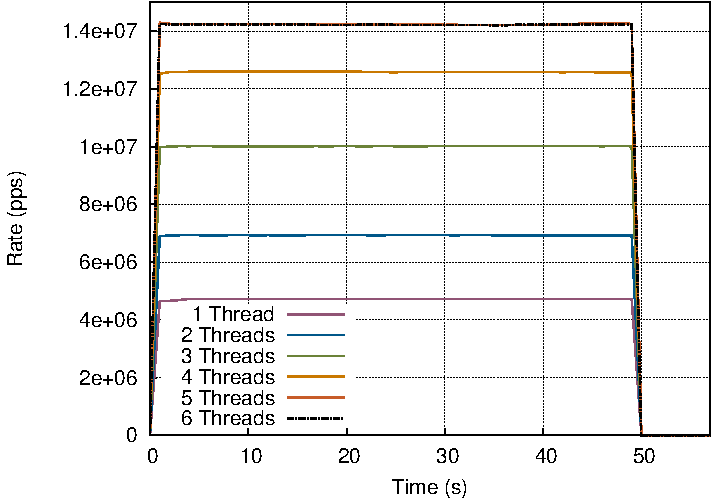
\includegraphics[width=\linewidth]{threads_vs_send.pdf}
\caption{\textbf{Threads vs.\ Scan Rate}\,---\,%
The send rate scales with the number of threads until reaching five threads,
at which point one thread is assigned per physical CPU. As threads begin to
share the same CPU, the send rate peaks. Using six threads results in an
identical send rate to five threads.
}
\label{fig:threads}
\end{figure}
\fi

\if0
\paragraph{Benchmarks}
We compared zero-copy NIC access to ZMap's traditional packet sending
architecture. In each case we also enabled the enhancements discussed in
Section~\ref{sec:TK} and Section~\ref{sec:TK} and conducted repeated scans of
covering 2\% samples of the public IPv4 address space. The average
transmission rate improved from 2.6~Mpps to 14.23~Mpps, a 447\% improvement.
This is 96\% of the theoretical limit of 10\,GigE,
14.88~Mpps~\cite{ten-gig-commodity}.
\fi

\begin{table}\centering
    \begin{tabular}{lrr}
    \toprule
    \textbf{Scan Rate} & \textbf{Hit Rate} & \textbf{Duration} \\ \midrule
    1.44 Mpps ($\approx$1\,GigE)                 & 1.00  & 42:08               \\ 
    3.00 Mpps                  & 0.99  & 20:47              \\ 
    4.00 Mpps                  & 0.97  & 15:38              \\
    14.23 Mpps ($\approx$10\,GigE)                 &  0.63 &  4:29               \\ % raw is 0.675
    \bottomrule
    \end{tabular}
    % 0.675
\caption{\textbf{Performance of Internet-wide Scans}\,---\,%
We show the scan rate, the normalized hit rate, and the scan duration (m:s)
for complete Internet-wide scans performed with optimized ZMap.}
\label{tbl:fullhitrate}
\end{table}

\section{Evaluation}
\label{sec:evaluation}

We performed a series of experiments to characterize the behavior of scanning
at speeds greater than 1~Gbps. In our test setup, we completed a full scan of
the public IPv4 address space in 4m29s on a server with a 10\,GigE uplink.
However, at full speed the number of scan results (the hit rate) decreased by
37\% compared to a scan at 1~Gbps, due to random packet drop. We find that we
can scan at speeds of up to 2.7~Gbps before seeing a substantial drop in hit
rate.

We performed the following measurements on a Dell PowerEdge R720 with two
Intel Xeon E5-2690 2.9~GHz processors (8 physical cores each plus
hyper-threading) and 128~GB of memory running Ubuntu 12.04.4~LTS and the
3.2.0-59-generic Linux kernel. We use a single port on a Intel X540-AT2
(rev~01) 10\,GigE controller as our scan interface, using the PF\_RING-aware
\texttt{ixgbe} driver bundled with PF\_RING 6.0.1. We configured ZMap to use
one send thread, one receive thread, one monitor thread, and five packet
creation threads.

We used a 10\,GigE network connection at the University of Michigan Computer
Science and Engineering division connected directly to the building uplink,
an aggregated $2\times 10$\,GigE channel. Beyond the 10\,GigE connection, the
only special network configuration arranged was static IP addresses. We note
that ZMap's performance may be different on other networks depending on local
congestion and upstream network conditions.\looseness=1

We performed all of our experiments using our local blacklist file. Our
blacklist, which eliminates non-routable address space and networks that have
requested exclusion from scanning~\cite{state-of-scanning}, consists of over
1,000 entries of various-sized network blocks. It results in 3.7~billion
allowed addresses---with almost all the excluded space consisting of IANA
reserved allocations.

\subsection{Hit-rate vs.\ Scan-rate}

In our original ZMap study, we experimented with various scanning speeds up
to gigabit Ethernet line speed (1.44~Mpps) and found no significant effect on
the number of results ZMap found~\cite{zmap}. In other words, from our
network, ZMap did not appear to miss any results when it ran faster up to
gigabit speed.

In order to determine whether hit-rate decreases with speeds higher than
1~Gigabit, we performed 50~second scans at speeds ranging from 0.1--14~Mpps.
We performed 3~trials at each scan rate. As can be seen in
Figure~\ref{fig:hitrate}, hit-rate begins to drop linearly after 4~Mpps. At
14~Mpps (close to 10\,GigE linespeed), the hit rate is 68\% of the hit rate
for a 1\,GigE scan. However, it is not immediately clear why this packet drop
is occurring at these higher speeds---are probe packets dropped by the
network, responses dropped by the network, or packets dropped on the scan
host due to ZMap?

\begin{figure}[t]\centering
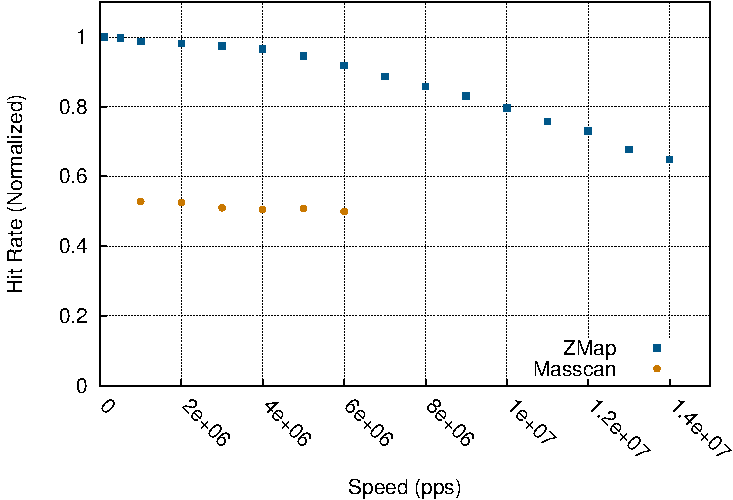
\includegraphics[height=2.1in]{\ZippyFigures/norm_avg_hitrate.pdf}
\caption{\textbf{Hit-rate vs.\ Scan-rate}\,---\,%
ZMap's hit rate is roughly stable up to a scan rate of 4~Mpps, then declines
linearly. This drop off may be due to upstreudegrm network congestion. Even using
PF\_RING, Masscan is unable to achieve scan rates above 6.4~Mpps on the same
hardware and has a much lower hit rate.}
\label{fig:hitrate}
\end{figure}

\begin{figure}[t]\centering
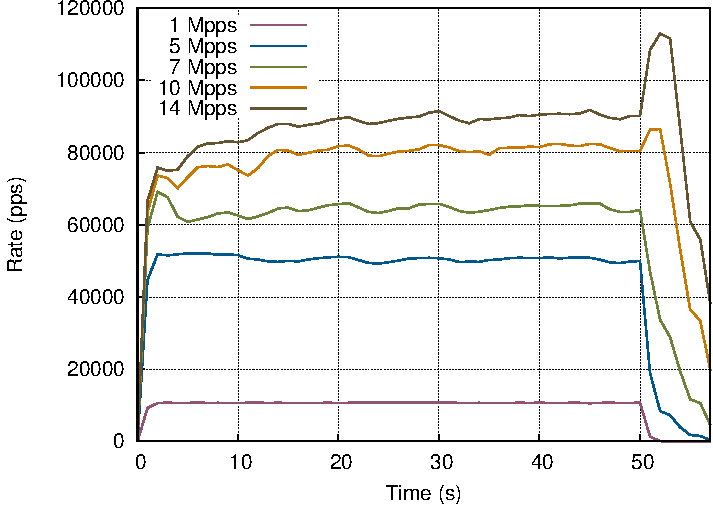
\includegraphics[height=2.1in]{\ZippyFigures/avg_count_recv_succs.pdf}
\caption{\textbf{Response Rate During Scans}\,---\,%
This graph shows the rate of incoming SYN-ACKs during 50-second scans. The
peaks at the end (after sending finishes) at rates above 7~Mpps indicate that
many responses are being dropped and retransmitted before being recorded by
ZMap.}
\label{fig:recvrate}
\end{figure}

We first investigate whether response packets are being dropped by ZMap or
the network. In the original ZMap work, we found that 99\% of hosts respond
within 1~second~\cite{zmap}. As such, we would expect that after 1~second,
there would be negligible responses. However, as can be seen in
Figure~\ref{fig:recvrate}, there is an unexpected spike in response packets
after sending completes at 50~seconds for scans at 10 and 14~Mpps. This spike
likely indicates that response packets are being dropped by our network, NIC,
or ZMap, as destination hosts will resend SYN-ACK packets for more than one
minute if an ACK or RST packet is not received.

In order to determine whether the drop of response packets is due to ZMap
inefficiencies or upstream network congestion, we performed a secondary scan
in which we split the probe generation and address processing onto separate
machines. The send machine remained the same. The receive machine was an HP
ProLiant DL120 G7, with an Intel Xeon E3-1230 processor (4 cores with
hyperthreading) and 16~GB of memory, running Ubuntu 12.04.4~LTS and the
3.5.0-52-generic Linux kernel.

As we show in Figure~\ref{fig:twomachines}, this spike does not occur when
processing response packets on a secondary server---instead it closely
follows the pattern of the slower scans. This indicates that ZMap is locally
dropping response packets. However, the split setup received only 4.3\% more
packets than the single machine---not enough to account for the 31.7\%
difference between a 14~Mpps and a 1~Mpps scan. If a large number of response
packets were dropped due to network congestion, we would not have observed an
immediate drop in responses---likely indicating that the root cause of the
decreased hit-rate is dropped probe packets.

It is not immediately clear where probe packets are dropped---it is possible
that packets are dropped locally by PF\_RING, are dropped by local routers
due to congestion, or that we are overwhelming destination networks. PF\_RING
records locally dropped packets, which remained zero throughout our scans,
which indicates that packets are not being dropped locally. In order to
locate where packet drop is occurring on our network, we calculated the drop
rate per AS and found little AS-level correlation for packets dropped by the
10\,GigE scans, which suggests that random packet drop is occurring close to
our network rather than at particular distant destination networks.

\begin{figure}\centering
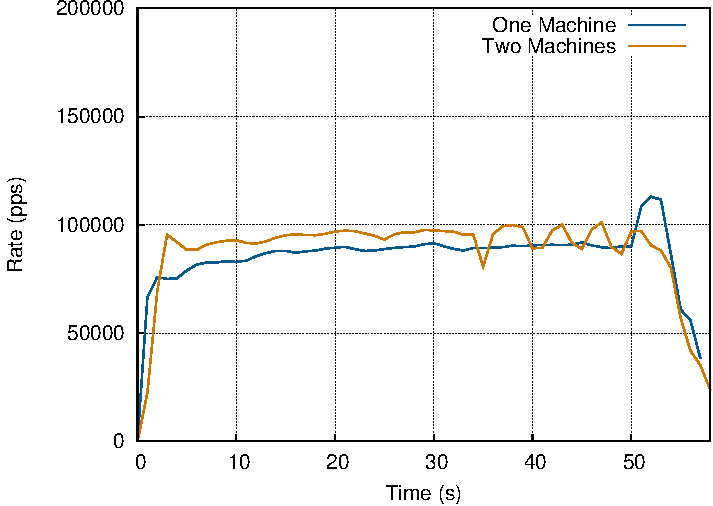
\includegraphics[width=\linewidth]{\ZippyFigures/split_avg_count_recv_succs.pdf}
\caption{\textbf{Comparing One and Two Machines}\,---\,%
If we scan at 14~Mpps and use separate machines for the sending and receiving
tasks, the spike in the SYN-ACK rate at 50~s disappears, indicating that
fewer packets are dropped with the workload spread over two machines.
However, overall the two machine configuration received only 4.3\% more
responses than with one machine, which suggests that network packet loss
accounts for the majority of the drop off at higher scan rates.}
\label{fig:twomachines}
\end{figure}

\subsection{Complete Scans}

We completed a full Internet-wide scan, allowing ZMap to operate at its full
scan rate. This scan achieved an average 14.23~Mpps---96\% of the theoretical
limit of 10\,GigE, completing in 4~minutes, 29~seconds and achieving a hit
rate that is 62.5\% of that from a 1\,GigE scan. We show a comparison to
lower speed scans in Table~\ref{tbl:fullhitrate}. As we discussed in the
previous section, this decrease is likely due to local network congestion,
which results in dropped probe packets. However, more investigation is
deserved in order to understand the full dynamics of high-speed scans.

\subsection{Comparison to Masscan}
\label{sec:masscan-comparison}

\begin{figure*}\centering
\hfill
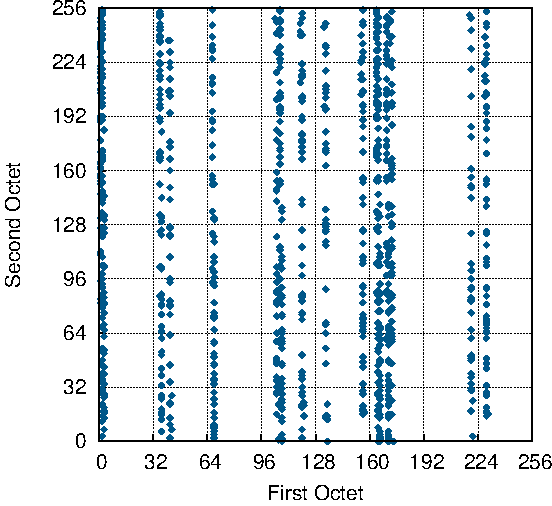
\includegraphics[height=2.5in]{\ZippyFigures/masscan_randomness.pdf}
\hfill\hfill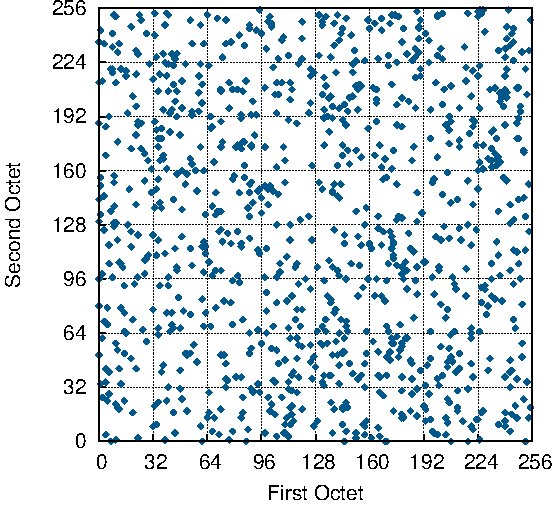
\includegraphics[height=2.5in]{\ZippyFigures/zmap_randomness.pdf}
\hfill\strut
\caption{\textbf{Address Randomization Comparison}\,---\,%
These plots depict the first 1000 addresses of an Internet-wide scan selected
by Masscan (\emph{left}) and ZMap (\emph{right}), with the first and second
octets mapped to the $x$ and~$y$ coordinates. ZMap's address randomization is
CPU intensive but achieves better statistical properties than the cheaper
approach used by Masscan, enabling valid sampling. We enhanced ZMap to
distribute address generation across multiple cores.}
\label{fig:randomy}
\end{figure*}

Masscan advertises the ability to emit probes at 25~Mpps using PF\_RING and
two 10\,GigE adapters, each configured with two RSS queues---84\% of
linespeed for dual 10\,GigE and 166\% of linespeed for a single 10\,GigE
adapter~\cite{masscan-10g}. We benchmarked ZMap and Masscan using the
Xeon~E3-1230 machine described above. In our experiments, we found that
Masscan was able to send at a peak 7.4~Mpps using a single-adapter
configuration with two RSS queues, 50\% of 10\,GigE linespeed. On the same
hardware, ZMap is capable of reaching a peak 14.1~Mpps. While Masscan may be
able to achieve a higher maximum speed using multiple adapters, ZMap is able
to fully saturate a 10\,GigE uplink with a single adapter.

Masscan uses a custom Feistel network to ``encrypt'' a monotonically
increasing index to generate a random permutation of the IPv4 address
space~\cite{masscan-rng}. While this is computation cheaper than using a
cyclic group, this technique results in poor statistical properties, which we
show in Figure~\ref{fig:randomy}. This has two consequences: first, it is not
suitable for sampling portions of the address space, and second, there is
greater potential for overloading destination networks. This could explain
the discrepency in Figure~\ref{fig:hitrate} if Masscan targeted a less
populated subnet.

Masscan and ZMap use a similar sharding approach to parallelize address
generation and distribute scans. Both programs ``count off'' addresses into
shards by staggering the offsets of the starting position of each shard
within the permutation and iterating a fixed number of steps through each of
their permutations. In ZMap, this is implemented by replacing the iteration
factor $g$ with $g^n$. In Masscan, this is simply a matter of incrementing
the monotonically increasing index by more than one.


\section{Applications}
\label{sec:discussion}

In this section, we consider applications that could benefit from 10\,GigE
scanning and remark on the implications of high-speed scanning for defenders
and attackers.

Scanning at faster rates reduces the blur introduced from hosts changing IP
addresses by decreasing the number of hosts that may be doubly counted during
longer scans. This also increases the ability to discover hosts that are only
online briefly. Thus, the ability to complete scans in minutes allows
researchers to more accurately create a snapshot of the Internet at a given
moment.

Similarly, the increased scan rate enables researchers to complete
high-resolution scans when measuring temporal effects. For example, while
researchers were able to complete comprehensive scans for the recent
Heartbleed Vulnerability every few hours~\cite{zmap-heartbleed}, many sites
were patched within the first minutes after disclosure. The ability to scan
more rapidly could help shed light on patching behavior within this critical
initial period.

\begin{figure*}
\centering
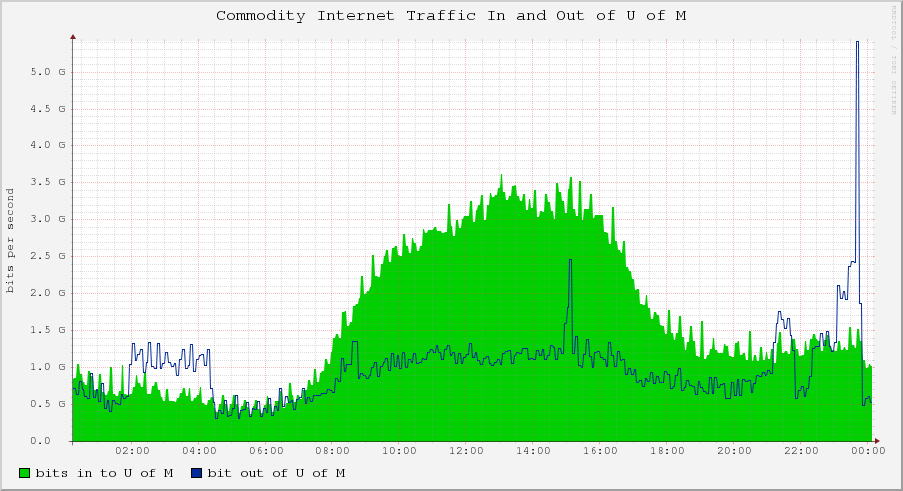
\includegraphics[width=0.75\linewidth]{\ZippyFigures/graph_image.png}
\caption{\textbf{10\,GigE   Scan Traffic}\,---\,%
An Internet-wide scan at full 10\,GigE speed dwarfed all other traffic at the
university during this 24~hour period. At 14.23~Mpps, a single machine
running ZMap generated 4.6~Gbps in outgoing IP traffic and scanned the entire
public IPv4 address space in 4m29s. The massive increase in outbound traffic
appears to have caused elevated packet drop. Notable smaller spikes are due
to earlier experiments.}
\label{fig:traffic}
\end{figure*}

Faster scan rates also allow for a variety of new scanning-related
applications that require multiple packets, including quickly completing
global trace routes or performing operating system fingerprinting.
Furthermore, the advancement of single-port scanning can be utilized to
quickly perform scans of a large number of ports, allowing scanning all
privileged ports on a /16 in under 5~seconds and \emph{all} ports in
5~minutes, assuming the attacker has sufficient bandwidth to the target.

The most alarming malicious potential for 10\,GigE scanning lies in its
ability to find and exploit vulnerabilities \emph{en masse} in a very short
time. Durumeric et~al.\ found that attackers began scanning for the
Heartbleed vulnerability within 22~hours of its
disclosure~\cite{zmap-heartbleed}. While attackers have utilized botnets and
worms in order to complete distributed scans for vulnerabilities, recent
work~\cite{state-of-scanning} has shown that attackers are now also using
ZMap, Masscan, and other scanning technology from bullet-proof hosting
providers in order to find vulnerable hosts. The increase in scan rates could
allow attackers to complete Internet-wide vulnerability scans in minutes as
10\,GigE becomes widely available.\looseness=-1

\section{Future Work}

We demonstrated that it is possible to perform Internet-wide scans at
10\,GigE linespeed, but, at least from our institutional network, we are
unable to sustain the expected hit rate as scanning approaches this packet
rate. Further investigation is needed to understand this effect and profile
ZMap's performance on other networks. One important question is whether the
drop off is caused by nearby network bottlenecks (which might be reduced with
upgraded network hardware) or whether it arises because such rapid scanning
induces congestion on many distant networks---which would represent an
inherent limit on scan speed. It is also possible that there are a small
number of remote bottlenecks that cause the observed drop in hit rate at high
speeds. In that case, identifying, profiling, and removing these bottlenecks
could improve performance.

40\,GigE hardware currently exists, and 100\,GigE is under
development~\cite{hundred-gig}. As these networks become more widely
available, it may be desirable to optimize and scale Internet-wide scanning
to even higher speeds.

\section{Conclusion}

In this work, we introduced enhancements to the ZMap Internet scanner that
enable it to scan at up to 14.2~Mpps. The three modifications we
present---sharding, optimized address constraints, and integration with
PF\_RING ZC---enable scanning at close to 10\,GigE linespeed. These
modifications are available now on experimental ZMap branches and will be
merged into mainline ZMap.

With these enhancements, we are able to complete a scan of the public IPv4
address space in 4m29s. However, despite having a well provisioned upstream
network, coverage in our experiments drops precipitously when scanning faster
than 4~Mpps. While further research is needed to better characterize and
reduce the causes of this drop off, it may be related to specific conditions
on our network.

As faster network infrastructure becomes more widely available, 10\,GigE
scanning will enable powerful new applications for both researchers and
attackers.

\section*{Acknowledgments}

The authors thank the exceptional sysadmins at the University of Michigan for
their help and support throughout this project. This research would not have
been possible without Kevin Cheek, Chris Brenner, Laura Fink, Paul Howell,
Don Winsor, and others from ITS, CAEN, and DCO\@. We are grateful to Michael
Bailey for numerous productive discussions, to Luca Deri and ntop for
providing a PF\_RING license, and to the many contributors to the ZMap open
source project. We also thank Denis Bueno, Jakub Czyz, Henry Fanson, Pat
Pannuto, and Eric Wustrow.

This material is based upon work supported by the National Science Foundation
under Grant No.~CNS-1255153 and No.~CNS-0964545. Any opinions, findings, and
conclusions or recommendations expressed in this material are those of the
authors and do not necessarily reflect the views of the National Science
Foundation.

%% !TEX root = ../../../proposal.tex

{\footnotesize\bibliographystyle{abbrv}
\balance
\bibliography{woot}}
\end{document}



\chapter{Drown}
%% !TEX root = ../../../proposal.tex

\newcommand*{\ZippyPaper}{papers/zippy/paper}
\newcommand*{\ZippyFigures}{papers/zippy/figures}
%% !TEX root = ../../../proposal.tex

\documentclass[letterpaper,twocolumn,10pt]{article}
\usepackage{usenix,epsfig,footnote,url}\urlstyle{rm}
\usepackage[T1]{fontenc}
\usepackage[%
    breaklinks=true,colorlinks=true,linkcolor=black,%
     citecolor=black,urlcolor=black,bookmarks=true,bookmarksopen=false,%
    pdfauthor={David Adrian, Zakir Durumeric, Gulshan Singh, and J. Alex Halderman},
    pdftitle={Zippier ZMap: Internet-Wide Scanning at 10 Gbps}
    ,pdftex]{hyperref}
\usepackage{amsmath, amssymb, amsfonts, amsthm}
\usepackage{mathptmx}\renewcommand{\ttdefault}{cmtt}
\usepackage[margin=0pt,font=small]{caption}
\usepackage{graphicx}
\usepackage{booktabs}
\usepackage{balance}
\usepackage{cite}
\usepackage[protrusion=true,expansion=true,kerning]{microtype}
\SetExtraKerning % Add space around emdashes
   { encoding = *,
        font = * }
   { \textemdash  = {120,120} }

% Fix ugly USENIX subsection headings (AH 3/08)
\makeatletter
\renewcommand{\section}{\@startsection {section}{1}{\z@}%
                                   {-3.5ex plus-1ex minus -.2ex}%
                                   {2.3ex plus.2ex}%
                                   {\normalfont\large\bfseries}}
\renewcommand{\subsection}{\@startsection{subsection}{2}{\z@}%
                                     {-2.5ex plus-.7ex minus -.2ex}%
                                     {1.5ex plus .2ex}%
                                     {\normalfont\fontsize{11}{12.5}\bfseries}}
\makeatother

% Paragraph and subpar
\renewcommand{\paragraph}[1]{\medskip\noindent\textbf{#1}\quad}
\newcommand{\subpar}[1]{\medskip\noindent\textsl{#1}\enspace}

% Stop URLs from hyphenating after  "http:" (AH 12/08)
\def\UrlBreaks{\do-\do\.\do\@\do\\\do\!\do\_\do\|\do\;\do\>\do\]%
 \do\)\do\,\do\?\do\'\do+\do\=\do\#}
\def\UrlBigBreaks{\do\:\do\/}%

% TODO, TK, etc. (AH 4/12)
\usepackage{xspace}
\newcommand{\todo}[1]{{\color{red}{\textbf{\em [TODO: #1]}}}\xspace}
\newcommand{\TODO}[1]{\todo{#1}}
\newcommand{\tk}{{\color{red}{\bf TK}}\xspace}
\newcommand{\TK}{\tk}
\newcommand{\comment}[1]{\relax} % comment out text
\newcommand{\xcite}[1]{\relax} % comment out citation

\newif\ifweb\webtrue
\ifweb
    \usepackage{watermark}
    \thiswatermark{\parbox{\textwidth}{\vskip30pt\centering
    \vspace*{-20pt}%
     This paper appeared in \emph{Proceedings of the 8th {USENIX} Workshop on Offensive Technologies} (WOOT '14), August~2014.\\
    \vskip6pt
    \rule[\baselineskip]{\textwidth}{0.5pt}
    }}
\fi

\begin{document}
\pagenumbering{arabic}
\thispagestyle{empty}

% Some math stuff
\newcommand{\bbZ}{\mathbb{Z}}

%don't want date printed
\date{}

\title{\Large\bf Zippier ZMap: Internet-Wide Scanning at 10\,Gbps}

\author{
{\rm David Adrian, Zakir Durumeric, Gulshan Singh, and J.\,Alex Halderman}\smallskip\\
University of Michigan\\
\small\rm\{davadria,\,zakir,\,gulshan,\,jhalderm\}@umich.edu
}
 

\maketitle


\begin{abstract}
We introduce optimizations to the ZMap network scanner that achieve a 10-fold
increase in maximum scan rate. By parallelizing address generation,
introducing an improved blacklisting algorithm, and using zero-copy NIC
access, we drive ZMap to nearly the maximum throughput of
10~gigabit~Ethernet, almost 15 million probes per second. With these changes,
ZMap can comprehensively scan for a single TCP port across the entire public
IPv4 address space in 4.5~minutes given adequate upstream bandwidth. We
consider the implications of such rapid scanning for both defenders and
attackers, and we briefly discuss a range of potential
applications.\looseness=1
\end{abstract}

\section{Introduction}
\label{sec:introduction}

In August 2013, we released ZMap, an open-source network scanner designed to
quickly perform Internet-wide network surveys~\cite{zmap}. From a single
machine, ZMap is capable of scanning at 1.44~million packets per second
(Mpps), the theoretical limit of gigabit Ethernet. At this speed, ZMap can
complete a scan targeting one TCP port across the entire public IPv4 address
space in under 45~minutes---a dramatic improvement compared to
weeks~\cite{zmap} or months~\cite{sslobservatory} required using Nmap. Yet
even at gigabit linespeed, ZMap does not utilize the full bandwidth of the
fastest readily available connections: 10\,GigE uplinks are now offered by
Amazon~EC2~\cite{amazon-10g} and at a growing number of research
institutions. \looseness=-1

In this paper, we scale ZMap to 10\,GigE speeds by introducing a series of
performance enhancements. These optimizations allow scanning speeds that
provide higher temporal resolution when conducting Internet-wide surveys and
make it possible to quickly complete complex multipacket studies.

Scanning at 10\,GigE linespeed necessitates sending nearly 15~Mpps
continuously. For single-packet probes such as SYN scans, this allows only
200 cycles per probe on a 3\,GHz core. An L2 cache miss might incur a cost of
almost 100 cycles, so it essential to make efficient use of both CPU and
memory. In order to generate and transmit packets at this rate, we introduce
modifications that target the three most expensive per-probe operations in
ZMap:
\begin{enumerate}
  \item \emph{Parallelized address generation.}\quad
    ZMap uses a multiplicative cyclic group to iterate over a random permutation
    of the address space, but this becomes a bottleneck at multigigabit speeds.
    We implement a mutex-free sharding mechanism that spreads address generation
    across multiple threads and cores.
  \item \emph{Optimized address constraints.}\quad
    Responsible scanning requires honoring requests from networks that opt out,
    but over time this can result in large and complex blacklists. We develop an
    optimized address constraint data structure that allows ZMap to efficiently
    cycle through allowed targets.
  \item \emph{Zero-copy packet transmission.}\quad
    ZMap sends Ethernet frames using a raw socket, which avoids the kernel's
    TCP/IP stack but still incurs a per-packet context switch. We switch to using
    the PF\_RING Zero Copy (ZC) interface, which bypasses the kernel and reduces
    memory bandwidth.
\end{enumerate}

These enhancements enable ZMap to scan at 14.23~Mpps, 96\% of the theoretical
limit of 10\,GigE\@. In order to confirm these performance gains, we
completed a full scan of the IPv4 address space in 4m29s---to our knowledge,
the fastest Internet-wide scan yet reported.

The ability to scan at 10\,GigE speeds creates new opportunities for security
researchers. It allows for truer snapshots of the state of the Internet by
reducing error due to hosts that move or change during the scan. Likewise, it
enables more accurate measurement of time-critical phenomena, such as
vulnerability patching in the minutes and hours after public disclosure. On
the other hand, it raises the possibility that attackers could use 10\,GigE
to exploit vulnerabilities with alarming speed.

\section{Related Work}
\label{sec:relatedwork}

Many network scanning tools have been
introduced~\cite{scanrand,unicornscan,masscan-10g,nmap,zmap}, although until
recently most were designed for scanning small networks. One of the most
popular is Nmap~\cite{nmap}, a highly capable network exploration tool. Nmap
is well suited for vertical scans of small networks or individual hosts, but
the original ZMap implementation outperformed it on horizontal Internet-wide
scans by a factor of 1300~\cite{zmap}. Our enhancements to ZMap improve its
performance by another factor of ten.

ZMap is not the first Internet-wide scanner to use PF\_RING to send at speeds
greater than 1~Gbps. Masscan, released in September 2013, also utilizes
PF\_RING and claims the ability to scan at 25~Mpps using dual 10\,GigE
ports---84\% of the theoretical limit of dual 10\,GigE~\cite{masscan-10g}. We
present a more detailed comparison to Masscan in
Section~\ref{sec:masscan-comparison}. While the Masscan team did not have the
facilities to perform live network tests at rates higher than
100,000~pps~\cite{masscan-10g}, we report what we believe is the first
Internet-wide scan conducted at 10\,GigE speeds.

\section{Performance Optimizations}
\label{sec:optimizations}

ZMap achieves this performance based on a series of architectural choices
that are geared towards very large, high-speed scans~\cite{zmap}. It avoids
per-connection state by embedding tracking information in packet fields that
will be echoed by the remote host, using an approach similar to
SYN~cookies~\cite{bernstein1996syn}. It eschews timeouts and simplifies flow
control by scanning according to a random permutation of the address space.
Finally, it avoids the OS's TCP/IP stack and writes raw Ethernet frames.

This architecture allows ZMap to exceed gigabit Ethernet linespeed on
commodity hardware, but there are several bottlenecks that prevent it from
fully reaching 10\,GigE speeds. ZMap's address generation is CPU intensive
and requires a global lock, adding significant overhead. Blacklisting ranges
of addresses is expensive and scales poorly. Sending each packet requires a
context switch and unnecessary copies as packets are passed from userspace to
the kernel and then to the NIC~\cite{multi-core-network}. We implement
optimizations that reduce each of these bottlenecks.

\subsection{Address Generation Sharding}

Address generation in ZMap is designed to achieve two goals. First, it avoids
flooding destination networks by ordering targets according to a pseudorandom
permutation of the address space. Second, it enables statistically valid
sampling of the address space.
% by ensuring that prefixes of the permutation have good statistical
% randomness. However, on a per-probe basis, address generation is one of the
% most costly operations.

ZMap iterates over a multiplicative group of integers modulo $p$ that
represent 32-bit IPv4 addresses. By choosing $p$ to be $2^{32} + 15$, the
smallest prime larger than $2^{32}$, we guarantee that the group
$(\bbZ/p\bbZ)^{\times}$ is cyclic and that it covers the full IPv4 address
space. ZMap derives a new random primitive root $g$ for each scan in order to
generate new permutation of the address space. The scanner starts at a random
initial address $a_{0}$ and calculates $a_{i+1} = g \cdot a_{i} \bmod p$ to
iterate through the permutation. The iteration is complete when $a_{i+1}$
equals $a_{0}$.

The most expensive part of this scheme is the modulo operation, which must be
performed at every step of the iteration. Unfortunately, the modulo operation
cannot currently be performed by multiple threads at once, because each
address in the permutation is dependent on the previous---calculating the
next address requires acquiring a lock over the entire iterator state.

To remove this bottleneck and efficiently distribute address generation over
multiple cores, we extend ZMap to support sharding. In the context of ZMap, a
shard is a partition of the IPv4 address space that can be iterated over
independently from other shards; assigning one shard to each thread allows
for independent, mutex-free execution. Each shard contains a disjoint subset
of the group, with the union of all the shards covering the entire group.

To define $n$ shards, we choose an initial random address $a_0$ and assign
each sequential address $a_j$ in the permutation to shard $j \bmod n$. To
implement this, we initialize shards $1 \dots n$ with starting addresses
$a_0,\dots,a_{n-1}$, which can be efficiently calculated as $a_0 \cdot
g^{0,\dots,n-1}$. To iterate, we replace $g$ with $g^n$, which ``skips
forward'' in the permutation by $n$ elements at each step. Each shard
computes $a_{i+1} = a_i \cdot g^n \bmod p$ until reaching its shard specific
ending address $a_{e_j}$. For example, if there were three shards, the first
would scan
$\{ {a_0,\; a_3=g^3 \cdot a_0,\; a_6 = g^3 \cdot a_3,\dots,\; a_{e_1}} \}$,
second
$\{ {a_1,\; a_4=g^3 \cdot a_4,\; a_7 = g^3 \cdot a_4,\dots,\; a_{e_2}} \}$, 
and third 
$\{ {a_2,\; a_5=g^3 \cdot a_0,\; a_8 = g^3 \cdot a_5,\dots,\; a_{e_3}} \}$. 
We illustrate the process in Figure~\ref{fig:sharding}.

After pre-calculating the shard parameters, we only need to store three
integers per shard: the starting address $a_0$, the ending address $a_e$, and
the current address $a_i$. The iteration factor $g^n$ and modulus $p$ are the
same for all shards. Each thread can then iterate over a single shard
independently of the other threads, and no global lock is needed to determine
the next address to scan. Multiple shards can operate within the same ZMap
process as threads (the configuration we evaluate in this paper), or they can
be split across multiple machines in a distributed scanning mode.

\begin{figure}\centering
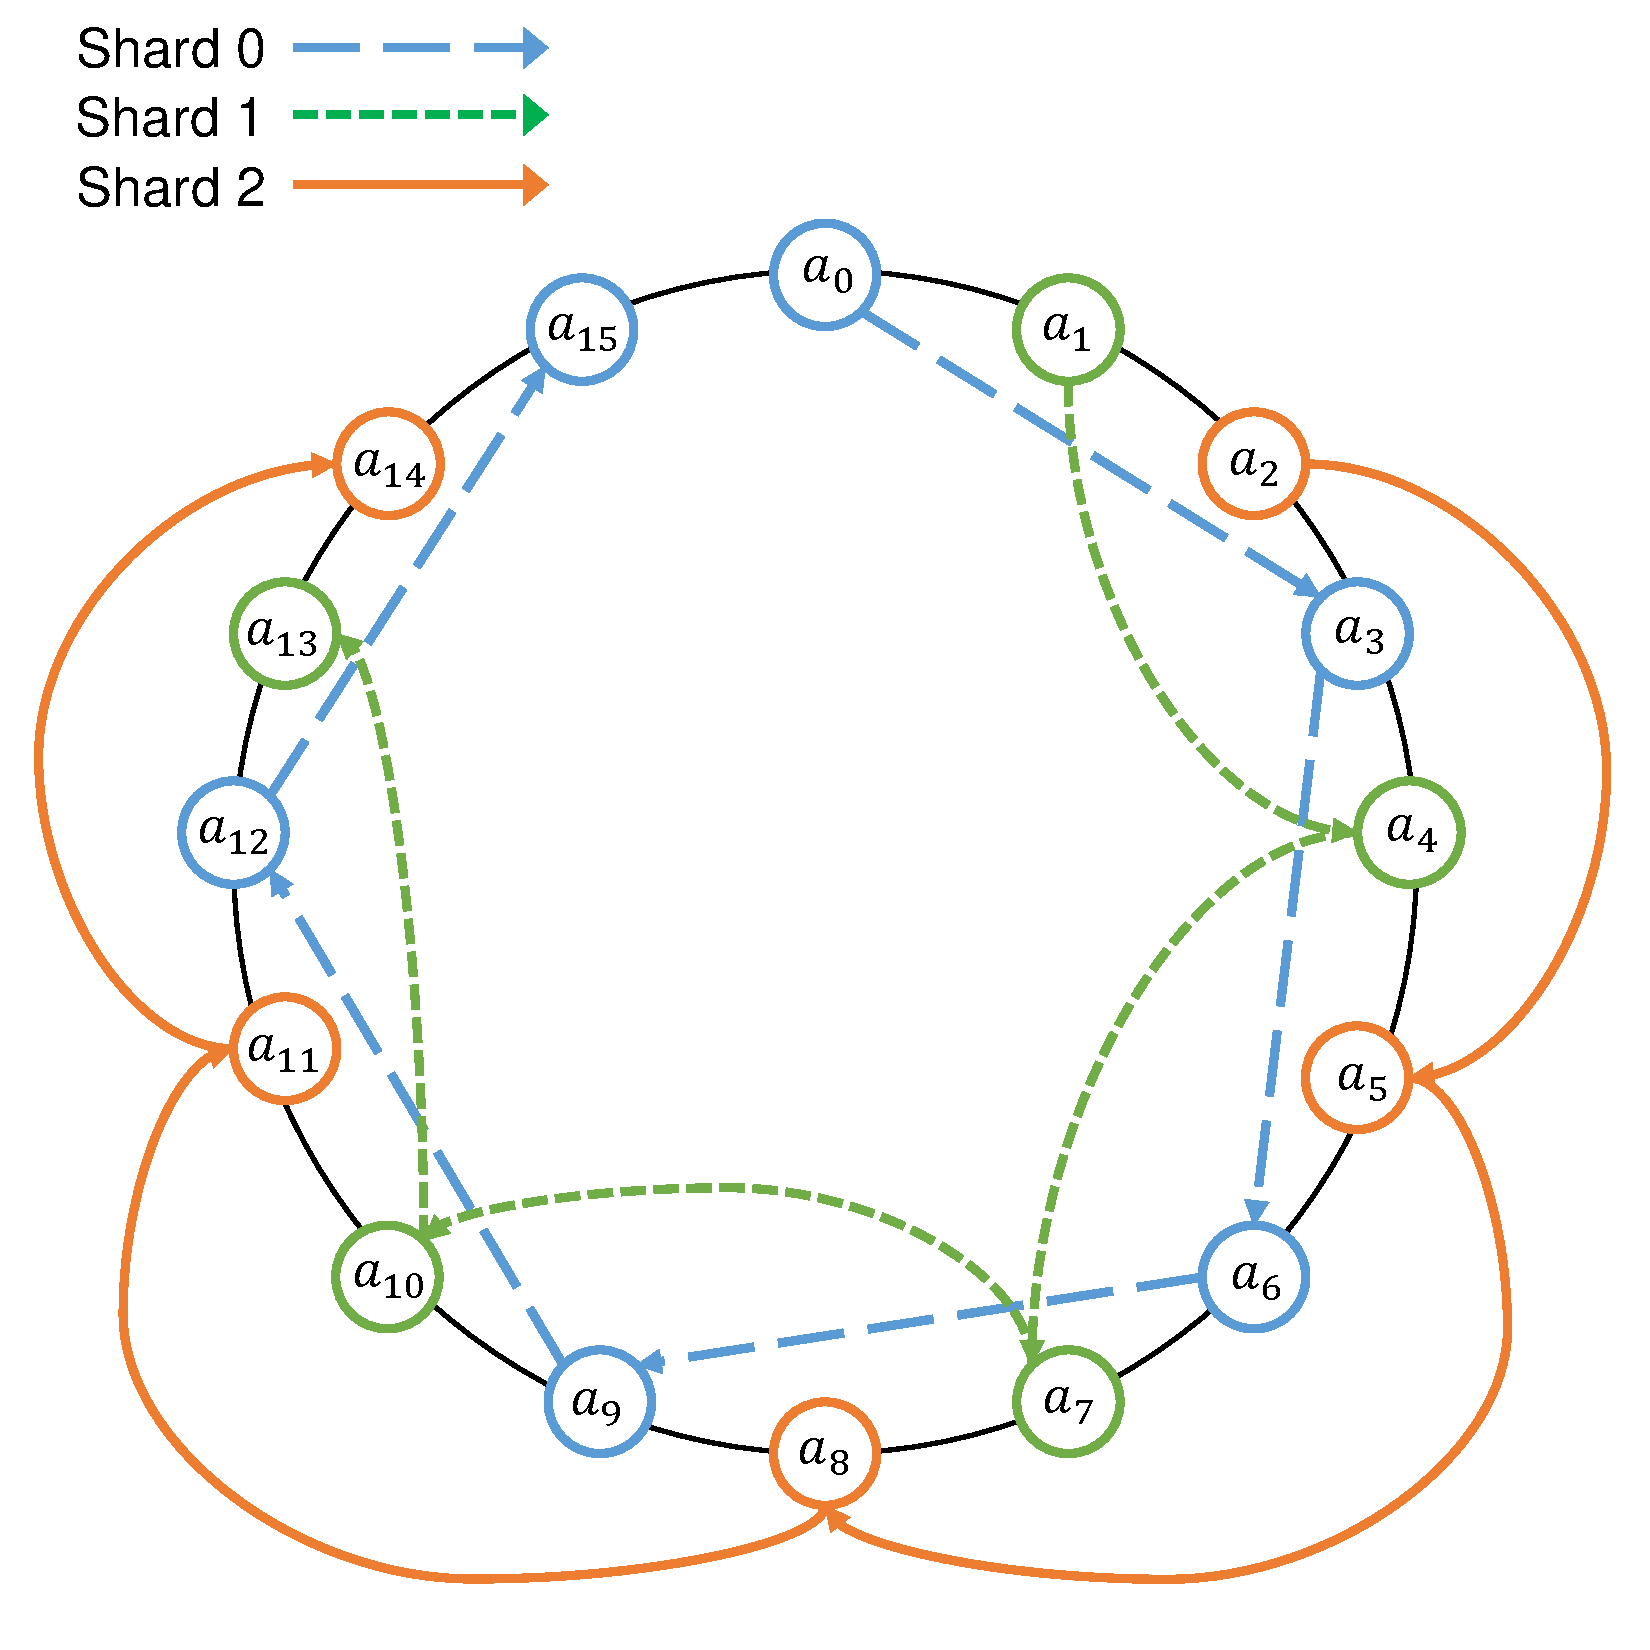
\includegraphics[width=\linewidth]{\ZippyFigures/shard_diagram.pdf}
\caption{\textbf{Sharding Visualization}\,---\,%
This is a configuration with three shards ($n = 3$). Shards $0,1,2$ are
initialized with starting addresses $a_0,a_1,a_2$. Each arrow represents
performing $a_i \cdot g^3$, a step forward by three elements in the
permutation.
}
\label{fig:sharding}
\end{figure}

\paragraph{Benchmarks}
To measure the impact of sharding in isolation from our other enhancements,
we conducted a series of scans, each covering a 1\% sample of the IP address
space, using our local blacklist file and a 10\,GigE uplink. Without
sharding, the average bandwidth utilization over 10~scans was 1.07 Gbps; with
sharding, the average increased to 1.80 Gbps, an improvement of 68\%.

\subsection{Blacklisting and Whitelisting}
 
ZMap address constraints are used to limit scans to specific areas of the
network (whitelisting) or to exclude particular address ranges
(blacklisting), such as IANA reserved allocations~\cite{iana}. Blacklisting
can also be used to comply with requests from network operators who want to
be excluded from receiving probe traffic. Good Internet citizenship demands
that ZMap users honor such requests, but after many scans over a prolonged
time period, a user's blacklist might contain hundreds of excluded prefixes.
 
Even with complicated address constraints, ZMap must be able to efficiently
determine whether any given IP address should be part of the scan. To support
10\,GigE linespeed, we implemented a combination tree- and array-based data
structure that can efficiently manipulate and query allowed addresses.

The IPv4 address space is modeled as a binary tree, where each node
corresponds to a network prefix. For example, the root represents 0.0.0.0/0,
and its children, if present, represent 0.0.0.0/1 and 128.0.0.0/1. Each
\emph{leaf} is colored either white or black, depending on whether or not the
corresponding prefix is allowed to be scanned. ZMap constructs the tree by
sequentially processing whitelist and blacklist entries that specify CIDR
prefixes. For each prefix, ZMap sets the color of the corresponding leaf,
adding new nodes or pruning the tree as necessary.

Querying whether an address may be scanned involves walking the tree,
beginning with the most significant bit of the address, until arriving at a
leaf and returning the color. However, a slightly different operation is used
during scanning. To make efficient use of the pseudorandom permutation
described above, we determine the number of allowed addresses $n$ (which may
be much smaller than the address space if a small whitelist is specified) and
select a permutation of approximately the same size. We then map from this
permutation of $1,\ldots,n$ to allowed addresses $a_1,\ldots,a_n$. Each node
in the tree maintains the total number of allowed addresses covered by its
descendants, allowing us to efficiently find the $i$th allowed address using
a simple recursive procedure.
%The ability to find specific addresses allows ZMap to utilize smaller cyclic
%groups to iterate over a small number of disjoint regions of address instead
%of iterating over the entire address space.\looseness=-1
 
As a further optimization, after the tree is constructed, we assemble a list
of /20 prefixes that are entirely allowed and reassign the address indices so
that these prefixes are ordered before any other allowed addresses. We then
use an array of these prefixes to optimize address lookups. If there are $m$
/20 prefixes that are allowed, then the first $m\cdot2^{12}$ allowed
addresses can be returned using only an array lookup, without needing to
consult the tree. The /20 size was determined empirically as a trade off
between lookup speed and memory usage.
 
\subsection{Zero-Copy NIC Access}
\label{sec:zc}
 
Despite ZMap's use of raw Ethernet sockets, sending each probe packet is an
expensive operation, as it involves a context switch for the \texttt{sendto}
system call and requires the scan packet to be transferred through kernel
space to the NIC~\cite{pfring-original, ten-gig-commodity}. Even with our
other enhancements, the high cost of these in-kernel operations prevented
ZMap from reaching above 2\,Gbps. To reduce these costs, we reimplemented
ZMap's network functionality using the PF\_RING ZC
interface~\cite{pfring-zc}. PF\_RING ZC allows userspace code to bypass the
kernel and have direct ``zero-copy'' access to the NIC\@, making it possible
to send packets without any context switches or wasted memory bandwidth.
 
To boost ZMap to 10\,GigE speeds, we implemented a new probe transmission
architecture on top of PF\_RING\@. This new architecture uses multiple
\emph{packet creation} threads that feed into a single \emph{send} thread. We
found that using more than one send thread for PF\_RING decreased the
performance of ZMap, but that a single packet creation thread was not fast
enough to reach line speed. By decoupling packet creation from sending, we
are able to combine the parallelization benefits of sharding with the speed
of PF\_RING\@.

In the original version of ZMap, multiple send threads each generated and
sent packets via a thread-specific raw Ethernet socket. We modify thread
responsibilities such that each packet creation thread iterates over one
address generation shard and generates and queues the packets. In a tight
loop, each packet generation loop calculates the next index in the shard,
finds the corresponding allowed IP address using the address constraint tree,
and creates an addressed packet in the PF\_RING ZC driver's memory. The
packet is added to a per-thread single-producer, single-consumer packet
queue. The send thread reads from each packet queue as packets come
available, and sends them over the wire using PF\_RING\@.

To determine the optimal number of packet creation threads, we performed a
series of tests, scanning for 50 seconds using 1--6 packet creation threads,
and measured the send rate. We find the optimal number of threads corresponds
with assigning one per physical core.
% Our results are show in Figure~\ref{fig:threads}.

\if0
\begin{figure}\centering
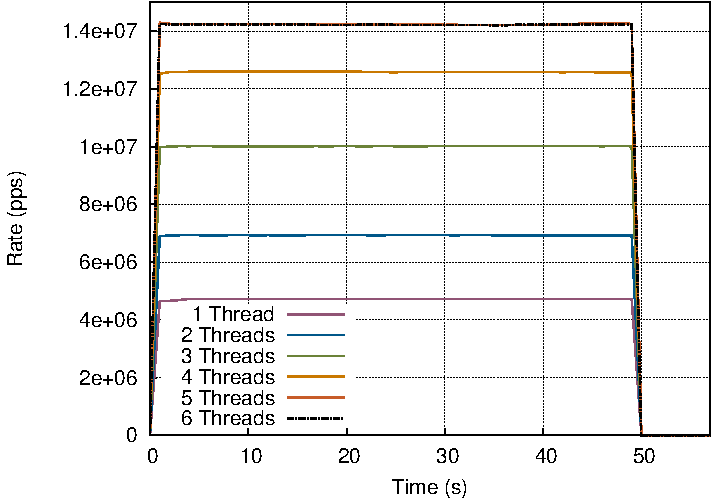
\includegraphics[width=\linewidth]{threads_vs_send.pdf}
\caption{\textbf{Threads vs.\ Scan Rate}\,---\,%
The send rate scales with the number of threads until reaching five threads,
at which point one thread is assigned per physical CPU. As threads begin to
share the same CPU, the send rate peaks. Using six threads results in an
identical send rate to five threads.
}
\label{fig:threads}
\end{figure}
\fi

\if0
\paragraph{Benchmarks}
We compared zero-copy NIC access to ZMap's traditional packet sending
architecture. In each case we also enabled the enhancements discussed in
Section~\ref{sec:TK} and Section~\ref{sec:TK} and conducted repeated scans of
covering 2\% samples of the public IPv4 address space. The average
transmission rate improved from 2.6~Mpps to 14.23~Mpps, a 447\% improvement.
This is 96\% of the theoretical limit of 10\,GigE,
14.88~Mpps~\cite{ten-gig-commodity}.
\fi

\begin{table}\centering
    \begin{tabular}{lrr}
    \toprule
    \textbf{Scan Rate} & \textbf{Hit Rate} & \textbf{Duration} \\ \midrule
    1.44 Mpps ($\approx$1\,GigE)                 & 1.00  & 42:08               \\ 
    3.00 Mpps                  & 0.99  & 20:47              \\ 
    4.00 Mpps                  & 0.97  & 15:38              \\
    14.23 Mpps ($\approx$10\,GigE)                 &  0.63 &  4:29               \\ % raw is 0.675
    \bottomrule
    \end{tabular}
    % 0.675
\caption{\textbf{Performance of Internet-wide Scans}\,---\,%
We show the scan rate, the normalized hit rate, and the scan duration (m:s)
for complete Internet-wide scans performed with optimized ZMap.}
\label{tbl:fullhitrate}
\end{table}

\section{Evaluation}
\label{sec:evaluation}

We performed a series of experiments to characterize the behavior of scanning
at speeds greater than 1~Gbps. In our test setup, we completed a full scan of
the public IPv4 address space in 4m29s on a server with a 10\,GigE uplink.
However, at full speed the number of scan results (the hit rate) decreased by
37\% compared to a scan at 1~Gbps, due to random packet drop. We find that we
can scan at speeds of up to 2.7~Gbps before seeing a substantial drop in hit
rate.

We performed the following measurements on a Dell PowerEdge R720 with two
Intel Xeon E5-2690 2.9~GHz processors (8 physical cores each plus
hyper-threading) and 128~GB of memory running Ubuntu 12.04.4~LTS and the
3.2.0-59-generic Linux kernel. We use a single port on a Intel X540-AT2
(rev~01) 10\,GigE controller as our scan interface, using the PF\_RING-aware
\texttt{ixgbe} driver bundled with PF\_RING 6.0.1. We configured ZMap to use
one send thread, one receive thread, one monitor thread, and five packet
creation threads.

We used a 10\,GigE network connection at the University of Michigan Computer
Science and Engineering division connected directly to the building uplink,
an aggregated $2\times 10$\,GigE channel. Beyond the 10\,GigE connection, the
only special network configuration arranged was static IP addresses. We note
that ZMap's performance may be different on other networks depending on local
congestion and upstream network conditions.\looseness=1

We performed all of our experiments using our local blacklist file. Our
blacklist, which eliminates non-routable address space and networks that have
requested exclusion from scanning~\cite{state-of-scanning}, consists of over
1,000 entries of various-sized network blocks. It results in 3.7~billion
allowed addresses---with almost all the excluded space consisting of IANA
reserved allocations.

\subsection{Hit-rate vs.\ Scan-rate}

In our original ZMap study, we experimented with various scanning speeds up
to gigabit Ethernet line speed (1.44~Mpps) and found no significant effect on
the number of results ZMap found~\cite{zmap}. In other words, from our
network, ZMap did not appear to miss any results when it ran faster up to
gigabit speed.

In order to determine whether hit-rate decreases with speeds higher than
1~Gigabit, we performed 50~second scans at speeds ranging from 0.1--14~Mpps.
We performed 3~trials at each scan rate. As can be seen in
Figure~\ref{fig:hitrate}, hit-rate begins to drop linearly after 4~Mpps. At
14~Mpps (close to 10\,GigE linespeed), the hit rate is 68\% of the hit rate
for a 1\,GigE scan. However, it is not immediately clear why this packet drop
is occurring at these higher speeds---are probe packets dropped by the
network, responses dropped by the network, or packets dropped on the scan
host due to ZMap?

\begin{figure}[t]\centering
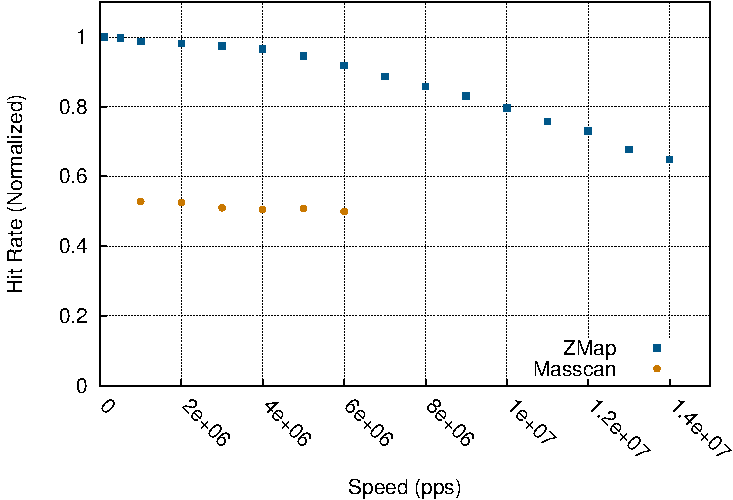
\includegraphics[height=2.1in]{\ZippyFigures/norm_avg_hitrate.pdf}
\caption{\textbf{Hit-rate vs.\ Scan-rate}\,---\,%
ZMap's hit rate is roughly stable up to a scan rate of 4~Mpps, then declines
linearly. This drop off may be due to upstreudegrm network congestion. Even using
PF\_RING, Masscan is unable to achieve scan rates above 6.4~Mpps on the same
hardware and has a much lower hit rate.}
\label{fig:hitrate}
\end{figure}

\begin{figure}[t]\centering
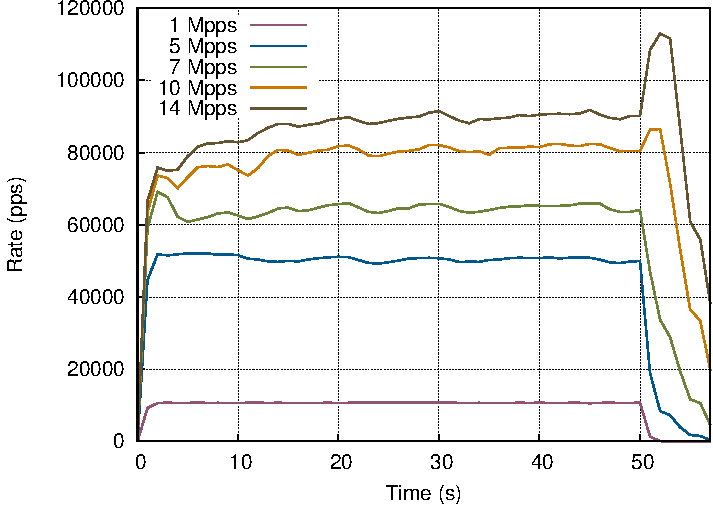
\includegraphics[height=2.1in]{\ZippyFigures/avg_count_recv_succs.pdf}
\caption{\textbf{Response Rate During Scans}\,---\,%
This graph shows the rate of incoming SYN-ACKs during 50-second scans. The
peaks at the end (after sending finishes) at rates above 7~Mpps indicate that
many responses are being dropped and retransmitted before being recorded by
ZMap.}
\label{fig:recvrate}
\end{figure}

We first investigate whether response packets are being dropped by ZMap or
the network. In the original ZMap work, we found that 99\% of hosts respond
within 1~second~\cite{zmap}. As such, we would expect that after 1~second,
there would be negligible responses. However, as can be seen in
Figure~\ref{fig:recvrate}, there is an unexpected spike in response packets
after sending completes at 50~seconds for scans at 10 and 14~Mpps. This spike
likely indicates that response packets are being dropped by our network, NIC,
or ZMap, as destination hosts will resend SYN-ACK packets for more than one
minute if an ACK or RST packet is not received.

In order to determine whether the drop of response packets is due to ZMap
inefficiencies or upstream network congestion, we performed a secondary scan
in which we split the probe generation and address processing onto separate
machines. The send machine remained the same. The receive machine was an HP
ProLiant DL120 G7, with an Intel Xeon E3-1230 processor (4 cores with
hyperthreading) and 16~GB of memory, running Ubuntu 12.04.4~LTS and the
3.5.0-52-generic Linux kernel.

As we show in Figure~\ref{fig:twomachines}, this spike does not occur when
processing response packets on a secondary server---instead it closely
follows the pattern of the slower scans. This indicates that ZMap is locally
dropping response packets. However, the split setup received only 4.3\% more
packets than the single machine---not enough to account for the 31.7\%
difference between a 14~Mpps and a 1~Mpps scan. If a large number of response
packets were dropped due to network congestion, we would not have observed an
immediate drop in responses---likely indicating that the root cause of the
decreased hit-rate is dropped probe packets.

It is not immediately clear where probe packets are dropped---it is possible
that packets are dropped locally by PF\_RING, are dropped by local routers
due to congestion, or that we are overwhelming destination networks. PF\_RING
records locally dropped packets, which remained zero throughout our scans,
which indicates that packets are not being dropped locally. In order to
locate where packet drop is occurring on our network, we calculated the drop
rate per AS and found little AS-level correlation for packets dropped by the
10\,GigE scans, which suggests that random packet drop is occurring close to
our network rather than at particular distant destination networks.

\begin{figure}\centering
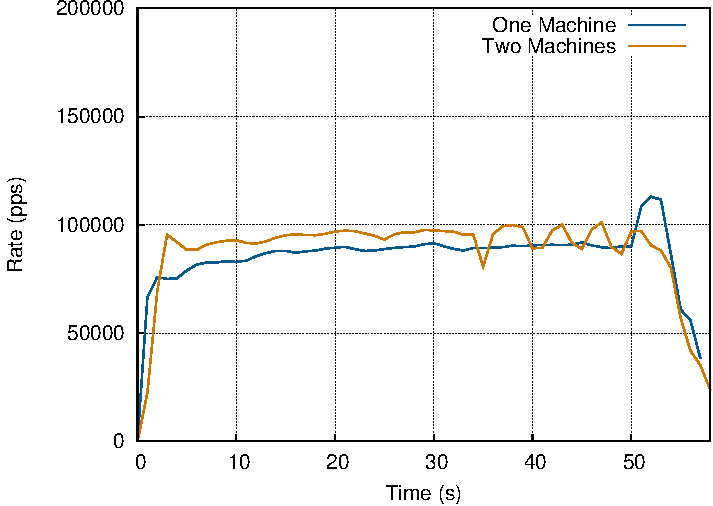
\includegraphics[width=\linewidth]{\ZippyFigures/split_avg_count_recv_succs.pdf}
\caption{\textbf{Comparing One and Two Machines}\,---\,%
If we scan at 14~Mpps and use separate machines for the sending and receiving
tasks, the spike in the SYN-ACK rate at 50~s disappears, indicating that
fewer packets are dropped with the workload spread over two machines.
However, overall the two machine configuration received only 4.3\% more
responses than with one machine, which suggests that network packet loss
accounts for the majority of the drop off at higher scan rates.}
\label{fig:twomachines}
\end{figure}

\subsection{Complete Scans}

We completed a full Internet-wide scan, allowing ZMap to operate at its full
scan rate. This scan achieved an average 14.23~Mpps---96\% of the theoretical
limit of 10\,GigE, completing in 4~minutes, 29~seconds and achieving a hit
rate that is 62.5\% of that from a 1\,GigE scan. We show a comparison to
lower speed scans in Table~\ref{tbl:fullhitrate}. As we discussed in the
previous section, this decrease is likely due to local network congestion,
which results in dropped probe packets. However, more investigation is
deserved in order to understand the full dynamics of high-speed scans.

\subsection{Comparison to Masscan}
\label{sec:masscan-comparison}

\begin{figure*}\centering
\hfill
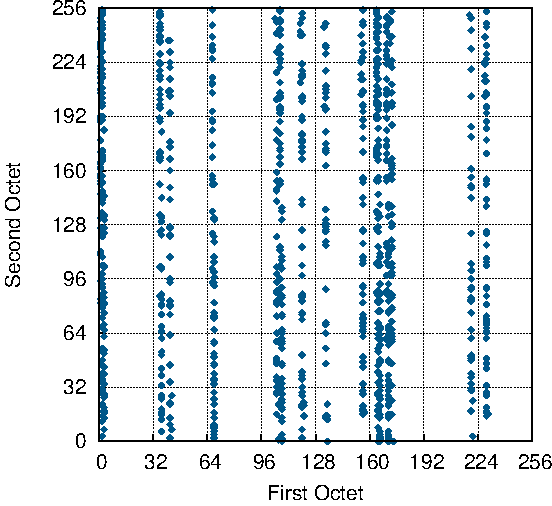
\includegraphics[height=2.5in]{\ZippyFigures/masscan_randomness.pdf}
\hfill\hfill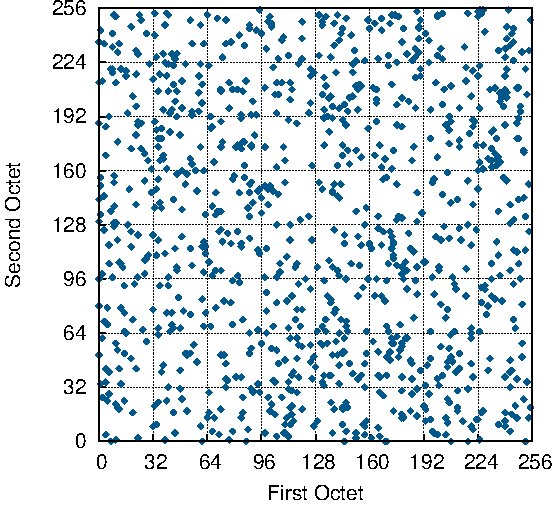
\includegraphics[height=2.5in]{\ZippyFigures/zmap_randomness.pdf}
\hfill\strut
\caption{\textbf{Address Randomization Comparison}\,---\,%
These plots depict the first 1000 addresses of an Internet-wide scan selected
by Masscan (\emph{left}) and ZMap (\emph{right}), with the first and second
octets mapped to the $x$ and~$y$ coordinates. ZMap's address randomization is
CPU intensive but achieves better statistical properties than the cheaper
approach used by Masscan, enabling valid sampling. We enhanced ZMap to
distribute address generation across multiple cores.}
\label{fig:randomy}
\end{figure*}

Masscan advertises the ability to emit probes at 25~Mpps using PF\_RING and
two 10\,GigE adapters, each configured with two RSS queues---84\% of
linespeed for dual 10\,GigE and 166\% of linespeed for a single 10\,GigE
adapter~\cite{masscan-10g}. We benchmarked ZMap and Masscan using the
Xeon~E3-1230 machine described above. In our experiments, we found that
Masscan was able to send at a peak 7.4~Mpps using a single-adapter
configuration with two RSS queues, 50\% of 10\,GigE linespeed. On the same
hardware, ZMap is capable of reaching a peak 14.1~Mpps. While Masscan may be
able to achieve a higher maximum speed using multiple adapters, ZMap is able
to fully saturate a 10\,GigE uplink with a single adapter.

Masscan uses a custom Feistel network to ``encrypt'' a monotonically
increasing index to generate a random permutation of the IPv4 address
space~\cite{masscan-rng}. While this is computation cheaper than using a
cyclic group, this technique results in poor statistical properties, which we
show in Figure~\ref{fig:randomy}. This has two consequences: first, it is not
suitable for sampling portions of the address space, and second, there is
greater potential for overloading destination networks. This could explain
the discrepency in Figure~\ref{fig:hitrate} if Masscan targeted a less
populated subnet.

Masscan and ZMap use a similar sharding approach to parallelize address
generation and distribute scans. Both programs ``count off'' addresses into
shards by staggering the offsets of the starting position of each shard
within the permutation and iterating a fixed number of steps through each of
their permutations. In ZMap, this is implemented by replacing the iteration
factor $g$ with $g^n$. In Masscan, this is simply a matter of incrementing
the monotonically increasing index by more than one.


\section{Applications}
\label{sec:discussion}

In this section, we consider applications that could benefit from 10\,GigE
scanning and remark on the implications of high-speed scanning for defenders
and attackers.

Scanning at faster rates reduces the blur introduced from hosts changing IP
addresses by decreasing the number of hosts that may be doubly counted during
longer scans. This also increases the ability to discover hosts that are only
online briefly. Thus, the ability to complete scans in minutes allows
researchers to more accurately create a snapshot of the Internet at a given
moment.

Similarly, the increased scan rate enables researchers to complete
high-resolution scans when measuring temporal effects. For example, while
researchers were able to complete comprehensive scans for the recent
Heartbleed Vulnerability every few hours~\cite{zmap-heartbleed}, many sites
were patched within the first minutes after disclosure. The ability to scan
more rapidly could help shed light on patching behavior within this critical
initial period.

\begin{figure*}
\centering
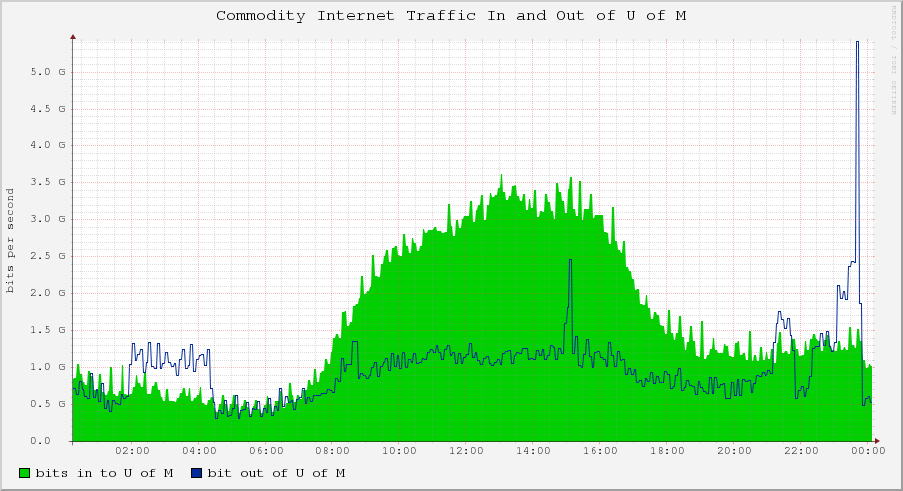
\includegraphics[width=0.75\linewidth]{\ZippyFigures/graph_image.png}
\caption{\textbf{10\,GigE   Scan Traffic}\,---\,%
An Internet-wide scan at full 10\,GigE speed dwarfed all other traffic at the
university during this 24~hour period. At 14.23~Mpps, a single machine
running ZMap generated 4.6~Gbps in outgoing IP traffic and scanned the entire
public IPv4 address space in 4m29s. The massive increase in outbound traffic
appears to have caused elevated packet drop. Notable smaller spikes are due
to earlier experiments.}
\label{fig:traffic}
\end{figure*}

Faster scan rates also allow for a variety of new scanning-related
applications that require multiple packets, including quickly completing
global trace routes or performing operating system fingerprinting.
Furthermore, the advancement of single-port scanning can be utilized to
quickly perform scans of a large number of ports, allowing scanning all
privileged ports on a /16 in under 5~seconds and \emph{all} ports in
5~minutes, assuming the attacker has sufficient bandwidth to the target.

The most alarming malicious potential for 10\,GigE scanning lies in its
ability to find and exploit vulnerabilities \emph{en masse} in a very short
time. Durumeric et~al.\ found that attackers began scanning for the
Heartbleed vulnerability within 22~hours of its
disclosure~\cite{zmap-heartbleed}. While attackers have utilized botnets and
worms in order to complete distributed scans for vulnerabilities, recent
work~\cite{state-of-scanning} has shown that attackers are now also using
ZMap, Masscan, and other scanning technology from bullet-proof hosting
providers in order to find vulnerable hosts. The increase in scan rates could
allow attackers to complete Internet-wide vulnerability scans in minutes as
10\,GigE becomes widely available.\looseness=-1

\section{Future Work}

We demonstrated that it is possible to perform Internet-wide scans at
10\,GigE linespeed, but, at least from our institutional network, we are
unable to sustain the expected hit rate as scanning approaches this packet
rate. Further investigation is needed to understand this effect and profile
ZMap's performance on other networks. One important question is whether the
drop off is caused by nearby network bottlenecks (which might be reduced with
upgraded network hardware) or whether it arises because such rapid scanning
induces congestion on many distant networks---which would represent an
inherent limit on scan speed. It is also possible that there are a small
number of remote bottlenecks that cause the observed drop in hit rate at high
speeds. In that case, identifying, profiling, and removing these bottlenecks
could improve performance.

40\,GigE hardware currently exists, and 100\,GigE is under
development~\cite{hundred-gig}. As these networks become more widely
available, it may be desirable to optimize and scale Internet-wide scanning
to even higher speeds.

\section{Conclusion}

In this work, we introduced enhancements to the ZMap Internet scanner that
enable it to scan at up to 14.2~Mpps. The three modifications we
present---sharding, optimized address constraints, and integration with
PF\_RING ZC---enable scanning at close to 10\,GigE linespeed. These
modifications are available now on experimental ZMap branches and will be
merged into mainline ZMap.

With these enhancements, we are able to complete a scan of the public IPv4
address space in 4m29s. However, despite having a well provisioned upstream
network, coverage in our experiments drops precipitously when scanning faster
than 4~Mpps. While further research is needed to better characterize and
reduce the causes of this drop off, it may be related to specific conditions
on our network.

As faster network infrastructure becomes more widely available, 10\,GigE
scanning will enable powerful new applications for both researchers and
attackers.

\section*{Acknowledgments}

The authors thank the exceptional sysadmins at the University of Michigan for
their help and support throughout this project. This research would not have
been possible without Kevin Cheek, Chris Brenner, Laura Fink, Paul Howell,
Don Winsor, and others from ITS, CAEN, and DCO\@. We are grateful to Michael
Bailey for numerous productive discussions, to Luca Deri and ntop for
providing a PF\_RING license, and to the many contributors to the ZMap open
source project. We also thank Denis Bueno, Jakub Czyz, Henry Fanson, Pat
Pannuto, and Eric Wustrow.

This material is based upon work supported by the National Science Foundation
under Grant No.~CNS-1255153 and No.~CNS-0964545. Any opinions, findings, and
conclusions or recommendations expressed in this material are those of the
authors and do not necessarily reflect the views of the National Science
Foundation.

%% !TEX root = ../../../proposal.tex

{\footnotesize\bibliographystyle{abbrv}
\balance
\bibliography{woot}}
\end{document}



\chapter{Subgroup}
%% !TEX root = ../../../proposal.tex

\newcommand*{\ZippyPaper}{papers/zippy/paper}
\newcommand*{\ZippyFigures}{papers/zippy/figures}
%% !TEX root = ../../../proposal.tex

\documentclass[letterpaper,twocolumn,10pt]{article}
\usepackage{usenix,epsfig,footnote,url}\urlstyle{rm}
\usepackage[T1]{fontenc}
\usepackage[%
    breaklinks=true,colorlinks=true,linkcolor=black,%
     citecolor=black,urlcolor=black,bookmarks=true,bookmarksopen=false,%
    pdfauthor={David Adrian, Zakir Durumeric, Gulshan Singh, and J. Alex Halderman},
    pdftitle={Zippier ZMap: Internet-Wide Scanning at 10 Gbps}
    ,pdftex]{hyperref}
\usepackage{amsmath, amssymb, amsfonts, amsthm}
\usepackage{mathptmx}\renewcommand{\ttdefault}{cmtt}
\usepackage[margin=0pt,font=small]{caption}
\usepackage{graphicx}
\usepackage{booktabs}
\usepackage{balance}
\usepackage{cite}
\usepackage[protrusion=true,expansion=true,kerning]{microtype}
\SetExtraKerning % Add space around emdashes
   { encoding = *,
        font = * }
   { \textemdash  = {120,120} }

% Fix ugly USENIX subsection headings (AH 3/08)
\makeatletter
\renewcommand{\section}{\@startsection {section}{1}{\z@}%
                                   {-3.5ex plus-1ex minus -.2ex}%
                                   {2.3ex plus.2ex}%
                                   {\normalfont\large\bfseries}}
\renewcommand{\subsection}{\@startsection{subsection}{2}{\z@}%
                                     {-2.5ex plus-.7ex minus -.2ex}%
                                     {1.5ex plus .2ex}%
                                     {\normalfont\fontsize{11}{12.5}\bfseries}}
\makeatother

% Paragraph and subpar
\renewcommand{\paragraph}[1]{\medskip\noindent\textbf{#1}\quad}
\newcommand{\subpar}[1]{\medskip\noindent\textsl{#1}\enspace}

% Stop URLs from hyphenating after  "http:" (AH 12/08)
\def\UrlBreaks{\do-\do\.\do\@\do\\\do\!\do\_\do\|\do\;\do\>\do\]%
 \do\)\do\,\do\?\do\'\do+\do\=\do\#}
\def\UrlBigBreaks{\do\:\do\/}%

% TODO, TK, etc. (AH 4/12)
\usepackage{xspace}
\newcommand{\todo}[1]{{\color{red}{\textbf{\em [TODO: #1]}}}\xspace}
\newcommand{\TODO}[1]{\todo{#1}}
\newcommand{\tk}{{\color{red}{\bf TK}}\xspace}
\newcommand{\TK}{\tk}
\newcommand{\comment}[1]{\relax} % comment out text
\newcommand{\xcite}[1]{\relax} % comment out citation

\newif\ifweb\webtrue
\ifweb
    \usepackage{watermark}
    \thiswatermark{\parbox{\textwidth}{\vskip30pt\centering
    \vspace*{-20pt}%
     This paper appeared in \emph{Proceedings of the 8th {USENIX} Workshop on Offensive Technologies} (WOOT '14), August~2014.\\
    \vskip6pt
    \rule[\baselineskip]{\textwidth}{0.5pt}
    }}
\fi

\begin{document}
\pagenumbering{arabic}
\thispagestyle{empty}

% Some math stuff
\newcommand{\bbZ}{\mathbb{Z}}

%don't want date printed
\date{}

\title{\Large\bf Zippier ZMap: Internet-Wide Scanning at 10\,Gbps}

\author{
{\rm David Adrian, Zakir Durumeric, Gulshan Singh, and J.\,Alex Halderman}\smallskip\\
University of Michigan\\
\small\rm\{davadria,\,zakir,\,gulshan,\,jhalderm\}@umich.edu
}
 

\maketitle


\begin{abstract}
We introduce optimizations to the ZMap network scanner that achieve a 10-fold
increase in maximum scan rate. By parallelizing address generation,
introducing an improved blacklisting algorithm, and using zero-copy NIC
access, we drive ZMap to nearly the maximum throughput of
10~gigabit~Ethernet, almost 15 million probes per second. With these changes,
ZMap can comprehensively scan for a single TCP port across the entire public
IPv4 address space in 4.5~minutes given adequate upstream bandwidth. We
consider the implications of such rapid scanning for both defenders and
attackers, and we briefly discuss a range of potential
applications.\looseness=1
\end{abstract}

\section{Introduction}
\label{sec:introduction}

In August 2013, we released ZMap, an open-source network scanner designed to
quickly perform Internet-wide network surveys~\cite{zmap}. From a single
machine, ZMap is capable of scanning at 1.44~million packets per second
(Mpps), the theoretical limit of gigabit Ethernet. At this speed, ZMap can
complete a scan targeting one TCP port across the entire public IPv4 address
space in under 45~minutes---a dramatic improvement compared to
weeks~\cite{zmap} or months~\cite{sslobservatory} required using Nmap. Yet
even at gigabit linespeed, ZMap does not utilize the full bandwidth of the
fastest readily available connections: 10\,GigE uplinks are now offered by
Amazon~EC2~\cite{amazon-10g} and at a growing number of research
institutions. \looseness=-1

In this paper, we scale ZMap to 10\,GigE speeds by introducing a series of
performance enhancements. These optimizations allow scanning speeds that
provide higher temporal resolution when conducting Internet-wide surveys and
make it possible to quickly complete complex multipacket studies.

Scanning at 10\,GigE linespeed necessitates sending nearly 15~Mpps
continuously. For single-packet probes such as SYN scans, this allows only
200 cycles per probe on a 3\,GHz core. An L2 cache miss might incur a cost of
almost 100 cycles, so it essential to make efficient use of both CPU and
memory. In order to generate and transmit packets at this rate, we introduce
modifications that target the three most expensive per-probe operations in
ZMap:
\begin{enumerate}
  \item \emph{Parallelized address generation.}\quad
    ZMap uses a multiplicative cyclic group to iterate over a random permutation
    of the address space, but this becomes a bottleneck at multigigabit speeds.
    We implement a mutex-free sharding mechanism that spreads address generation
    across multiple threads and cores.
  \item \emph{Optimized address constraints.}\quad
    Responsible scanning requires honoring requests from networks that opt out,
    but over time this can result in large and complex blacklists. We develop an
    optimized address constraint data structure that allows ZMap to efficiently
    cycle through allowed targets.
  \item \emph{Zero-copy packet transmission.}\quad
    ZMap sends Ethernet frames using a raw socket, which avoids the kernel's
    TCP/IP stack but still incurs a per-packet context switch. We switch to using
    the PF\_RING Zero Copy (ZC) interface, which bypasses the kernel and reduces
    memory bandwidth.
\end{enumerate}

These enhancements enable ZMap to scan at 14.23~Mpps, 96\% of the theoretical
limit of 10\,GigE\@. In order to confirm these performance gains, we
completed a full scan of the IPv4 address space in 4m29s---to our knowledge,
the fastest Internet-wide scan yet reported.

The ability to scan at 10\,GigE speeds creates new opportunities for security
researchers. It allows for truer snapshots of the state of the Internet by
reducing error due to hosts that move or change during the scan. Likewise, it
enables more accurate measurement of time-critical phenomena, such as
vulnerability patching in the minutes and hours after public disclosure. On
the other hand, it raises the possibility that attackers could use 10\,GigE
to exploit vulnerabilities with alarming speed.

\section{Related Work}
\label{sec:relatedwork}

Many network scanning tools have been
introduced~\cite{scanrand,unicornscan,masscan-10g,nmap,zmap}, although until
recently most were designed for scanning small networks. One of the most
popular is Nmap~\cite{nmap}, a highly capable network exploration tool. Nmap
is well suited for vertical scans of small networks or individual hosts, but
the original ZMap implementation outperformed it on horizontal Internet-wide
scans by a factor of 1300~\cite{zmap}. Our enhancements to ZMap improve its
performance by another factor of ten.

ZMap is not the first Internet-wide scanner to use PF\_RING to send at speeds
greater than 1~Gbps. Masscan, released in September 2013, also utilizes
PF\_RING and claims the ability to scan at 25~Mpps using dual 10\,GigE
ports---84\% of the theoretical limit of dual 10\,GigE~\cite{masscan-10g}. We
present a more detailed comparison to Masscan in
Section~\ref{sec:masscan-comparison}. While the Masscan team did not have the
facilities to perform live network tests at rates higher than
100,000~pps~\cite{masscan-10g}, we report what we believe is the first
Internet-wide scan conducted at 10\,GigE speeds.

\section{Performance Optimizations}
\label{sec:optimizations}

ZMap achieves this performance based on a series of architectural choices
that are geared towards very large, high-speed scans~\cite{zmap}. It avoids
per-connection state by embedding tracking information in packet fields that
will be echoed by the remote host, using an approach similar to
SYN~cookies~\cite{bernstein1996syn}. It eschews timeouts and simplifies flow
control by scanning according to a random permutation of the address space.
Finally, it avoids the OS's TCP/IP stack and writes raw Ethernet frames.

This architecture allows ZMap to exceed gigabit Ethernet linespeed on
commodity hardware, but there are several bottlenecks that prevent it from
fully reaching 10\,GigE speeds. ZMap's address generation is CPU intensive
and requires a global lock, adding significant overhead. Blacklisting ranges
of addresses is expensive and scales poorly. Sending each packet requires a
context switch and unnecessary copies as packets are passed from userspace to
the kernel and then to the NIC~\cite{multi-core-network}. We implement
optimizations that reduce each of these bottlenecks.

\subsection{Address Generation Sharding}

Address generation in ZMap is designed to achieve two goals. First, it avoids
flooding destination networks by ordering targets according to a pseudorandom
permutation of the address space. Second, it enables statistically valid
sampling of the address space.
% by ensuring that prefixes of the permutation have good statistical
% randomness. However, on a per-probe basis, address generation is one of the
% most costly operations.

ZMap iterates over a multiplicative group of integers modulo $p$ that
represent 32-bit IPv4 addresses. By choosing $p$ to be $2^{32} + 15$, the
smallest prime larger than $2^{32}$, we guarantee that the group
$(\bbZ/p\bbZ)^{\times}$ is cyclic and that it covers the full IPv4 address
space. ZMap derives a new random primitive root $g$ for each scan in order to
generate new permutation of the address space. The scanner starts at a random
initial address $a_{0}$ and calculates $a_{i+1} = g \cdot a_{i} \bmod p$ to
iterate through the permutation. The iteration is complete when $a_{i+1}$
equals $a_{0}$.

The most expensive part of this scheme is the modulo operation, which must be
performed at every step of the iteration. Unfortunately, the modulo operation
cannot currently be performed by multiple threads at once, because each
address in the permutation is dependent on the previous---calculating the
next address requires acquiring a lock over the entire iterator state.

To remove this bottleneck and efficiently distribute address generation over
multiple cores, we extend ZMap to support sharding. In the context of ZMap, a
shard is a partition of the IPv4 address space that can be iterated over
independently from other shards; assigning one shard to each thread allows
for independent, mutex-free execution. Each shard contains a disjoint subset
of the group, with the union of all the shards covering the entire group.

To define $n$ shards, we choose an initial random address $a_0$ and assign
each sequential address $a_j$ in the permutation to shard $j \bmod n$. To
implement this, we initialize shards $1 \dots n$ with starting addresses
$a_0,\dots,a_{n-1}$, which can be efficiently calculated as $a_0 \cdot
g^{0,\dots,n-1}$. To iterate, we replace $g$ with $g^n$, which ``skips
forward'' in the permutation by $n$ elements at each step. Each shard
computes $a_{i+1} = a_i \cdot g^n \bmod p$ until reaching its shard specific
ending address $a_{e_j}$. For example, if there were three shards, the first
would scan
$\{ {a_0,\; a_3=g^3 \cdot a_0,\; a_6 = g^3 \cdot a_3,\dots,\; a_{e_1}} \}$,
second
$\{ {a_1,\; a_4=g^3 \cdot a_4,\; a_7 = g^3 \cdot a_4,\dots,\; a_{e_2}} \}$, 
and third 
$\{ {a_2,\; a_5=g^3 \cdot a_0,\; a_8 = g^3 \cdot a_5,\dots,\; a_{e_3}} \}$. 
We illustrate the process in Figure~\ref{fig:sharding}.

After pre-calculating the shard parameters, we only need to store three
integers per shard: the starting address $a_0$, the ending address $a_e$, and
the current address $a_i$. The iteration factor $g^n$ and modulus $p$ are the
same for all shards. Each thread can then iterate over a single shard
independently of the other threads, and no global lock is needed to determine
the next address to scan. Multiple shards can operate within the same ZMap
process as threads (the configuration we evaluate in this paper), or they can
be split across multiple machines in a distributed scanning mode.

\begin{figure}\centering
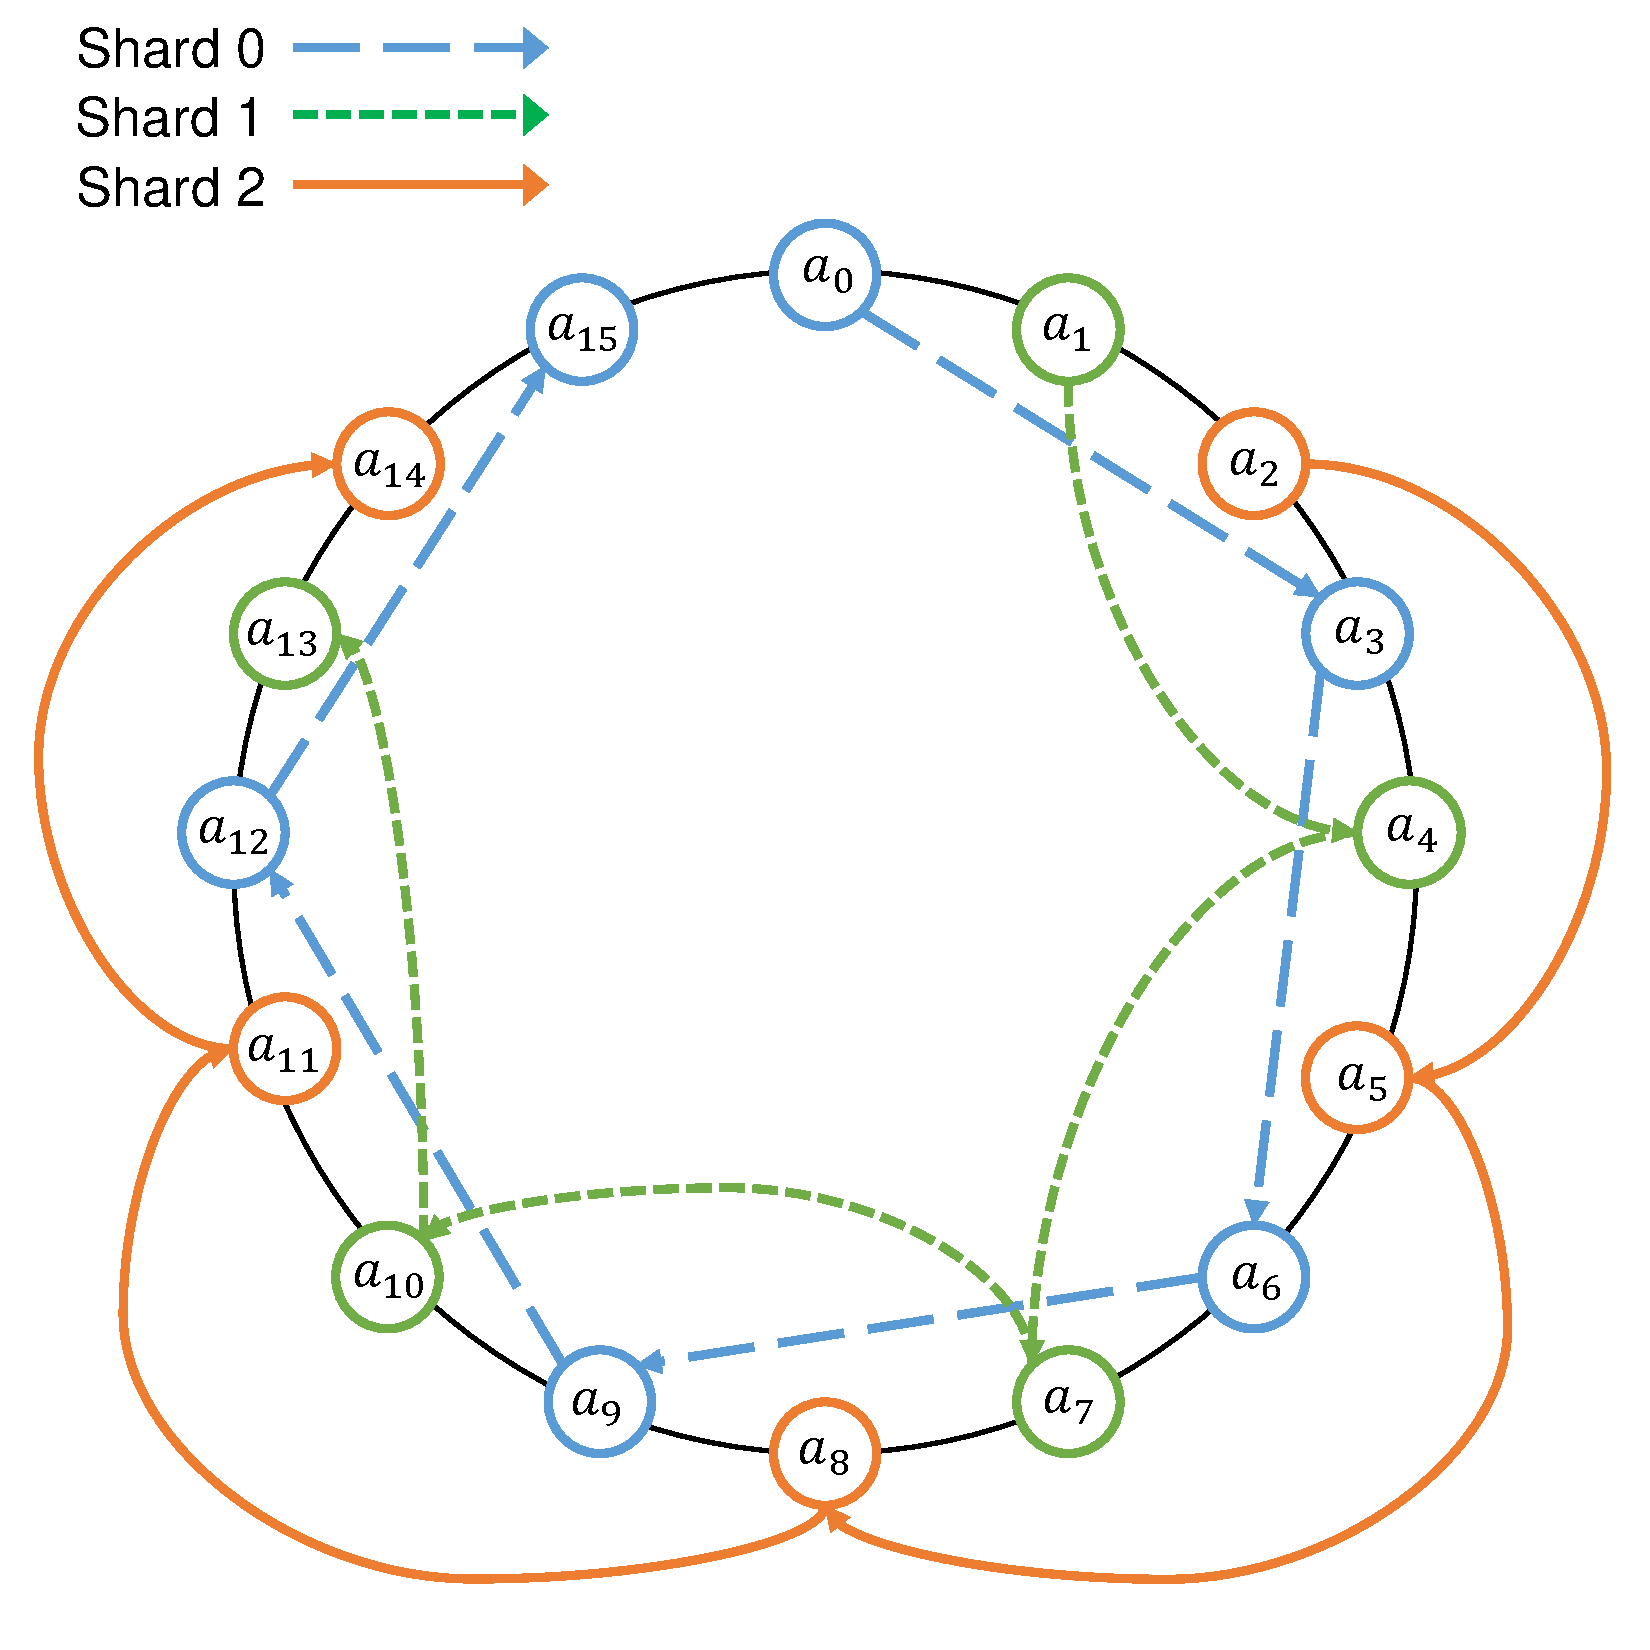
\includegraphics[width=\linewidth]{\ZippyFigures/shard_diagram.pdf}
\caption{\textbf{Sharding Visualization}\,---\,%
This is a configuration with three shards ($n = 3$). Shards $0,1,2$ are
initialized with starting addresses $a_0,a_1,a_2$. Each arrow represents
performing $a_i \cdot g^3$, a step forward by three elements in the
permutation.
}
\label{fig:sharding}
\end{figure}

\paragraph{Benchmarks}
To measure the impact of sharding in isolation from our other enhancements,
we conducted a series of scans, each covering a 1\% sample of the IP address
space, using our local blacklist file and a 10\,GigE uplink. Without
sharding, the average bandwidth utilization over 10~scans was 1.07 Gbps; with
sharding, the average increased to 1.80 Gbps, an improvement of 68\%.

\subsection{Blacklisting and Whitelisting}
 
ZMap address constraints are used to limit scans to specific areas of the
network (whitelisting) or to exclude particular address ranges
(blacklisting), such as IANA reserved allocations~\cite{iana}. Blacklisting
can also be used to comply with requests from network operators who want to
be excluded from receiving probe traffic. Good Internet citizenship demands
that ZMap users honor such requests, but after many scans over a prolonged
time period, a user's blacklist might contain hundreds of excluded prefixes.
 
Even with complicated address constraints, ZMap must be able to efficiently
determine whether any given IP address should be part of the scan. To support
10\,GigE linespeed, we implemented a combination tree- and array-based data
structure that can efficiently manipulate and query allowed addresses.

The IPv4 address space is modeled as a binary tree, where each node
corresponds to a network prefix. For example, the root represents 0.0.0.0/0,
and its children, if present, represent 0.0.0.0/1 and 128.0.0.0/1. Each
\emph{leaf} is colored either white or black, depending on whether or not the
corresponding prefix is allowed to be scanned. ZMap constructs the tree by
sequentially processing whitelist and blacklist entries that specify CIDR
prefixes. For each prefix, ZMap sets the color of the corresponding leaf,
adding new nodes or pruning the tree as necessary.

Querying whether an address may be scanned involves walking the tree,
beginning with the most significant bit of the address, until arriving at a
leaf and returning the color. However, a slightly different operation is used
during scanning. To make efficient use of the pseudorandom permutation
described above, we determine the number of allowed addresses $n$ (which may
be much smaller than the address space if a small whitelist is specified) and
select a permutation of approximately the same size. We then map from this
permutation of $1,\ldots,n$ to allowed addresses $a_1,\ldots,a_n$. Each node
in the tree maintains the total number of allowed addresses covered by its
descendants, allowing us to efficiently find the $i$th allowed address using
a simple recursive procedure.
%The ability to find specific addresses allows ZMap to utilize smaller cyclic
%groups to iterate over a small number of disjoint regions of address instead
%of iterating over the entire address space.\looseness=-1
 
As a further optimization, after the tree is constructed, we assemble a list
of /20 prefixes that are entirely allowed and reassign the address indices so
that these prefixes are ordered before any other allowed addresses. We then
use an array of these prefixes to optimize address lookups. If there are $m$
/20 prefixes that are allowed, then the first $m\cdot2^{12}$ allowed
addresses can be returned using only an array lookup, without needing to
consult the tree. The /20 size was determined empirically as a trade off
between lookup speed and memory usage.
 
\subsection{Zero-Copy NIC Access}
\label{sec:zc}
 
Despite ZMap's use of raw Ethernet sockets, sending each probe packet is an
expensive operation, as it involves a context switch for the \texttt{sendto}
system call and requires the scan packet to be transferred through kernel
space to the NIC~\cite{pfring-original, ten-gig-commodity}. Even with our
other enhancements, the high cost of these in-kernel operations prevented
ZMap from reaching above 2\,Gbps. To reduce these costs, we reimplemented
ZMap's network functionality using the PF\_RING ZC
interface~\cite{pfring-zc}. PF\_RING ZC allows userspace code to bypass the
kernel and have direct ``zero-copy'' access to the NIC\@, making it possible
to send packets without any context switches or wasted memory bandwidth.
 
To boost ZMap to 10\,GigE speeds, we implemented a new probe transmission
architecture on top of PF\_RING\@. This new architecture uses multiple
\emph{packet creation} threads that feed into a single \emph{send} thread. We
found that using more than one send thread for PF\_RING decreased the
performance of ZMap, but that a single packet creation thread was not fast
enough to reach line speed. By decoupling packet creation from sending, we
are able to combine the parallelization benefits of sharding with the speed
of PF\_RING\@.

In the original version of ZMap, multiple send threads each generated and
sent packets via a thread-specific raw Ethernet socket. We modify thread
responsibilities such that each packet creation thread iterates over one
address generation shard and generates and queues the packets. In a tight
loop, each packet generation loop calculates the next index in the shard,
finds the corresponding allowed IP address using the address constraint tree,
and creates an addressed packet in the PF\_RING ZC driver's memory. The
packet is added to a per-thread single-producer, single-consumer packet
queue. The send thread reads from each packet queue as packets come
available, and sends them over the wire using PF\_RING\@.

To determine the optimal number of packet creation threads, we performed a
series of tests, scanning for 50 seconds using 1--6 packet creation threads,
and measured the send rate. We find the optimal number of threads corresponds
with assigning one per physical core.
% Our results are show in Figure~\ref{fig:threads}.

\if0
\begin{figure}\centering
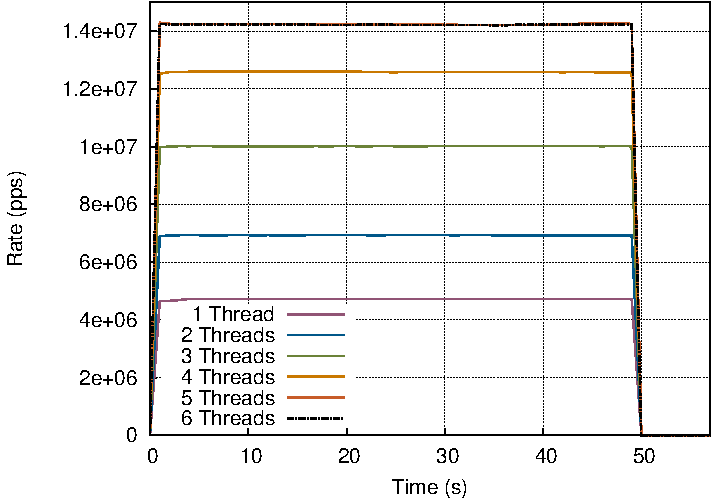
\includegraphics[width=\linewidth]{threads_vs_send.pdf}
\caption{\textbf{Threads vs.\ Scan Rate}\,---\,%
The send rate scales with the number of threads until reaching five threads,
at which point one thread is assigned per physical CPU. As threads begin to
share the same CPU, the send rate peaks. Using six threads results in an
identical send rate to five threads.
}
\label{fig:threads}
\end{figure}
\fi

\if0
\paragraph{Benchmarks}
We compared zero-copy NIC access to ZMap's traditional packet sending
architecture. In each case we also enabled the enhancements discussed in
Section~\ref{sec:TK} and Section~\ref{sec:TK} and conducted repeated scans of
covering 2\% samples of the public IPv4 address space. The average
transmission rate improved from 2.6~Mpps to 14.23~Mpps, a 447\% improvement.
This is 96\% of the theoretical limit of 10\,GigE,
14.88~Mpps~\cite{ten-gig-commodity}.
\fi

\begin{table}\centering
    \begin{tabular}{lrr}
    \toprule
    \textbf{Scan Rate} & \textbf{Hit Rate} & \textbf{Duration} \\ \midrule
    1.44 Mpps ($\approx$1\,GigE)                 & 1.00  & 42:08               \\ 
    3.00 Mpps                  & 0.99  & 20:47              \\ 
    4.00 Mpps                  & 0.97  & 15:38              \\
    14.23 Mpps ($\approx$10\,GigE)                 &  0.63 &  4:29               \\ % raw is 0.675
    \bottomrule
    \end{tabular}
    % 0.675
\caption{\textbf{Performance of Internet-wide Scans}\,---\,%
We show the scan rate, the normalized hit rate, and the scan duration (m:s)
for complete Internet-wide scans performed with optimized ZMap.}
\label{tbl:fullhitrate}
\end{table}

\section{Evaluation}
\label{sec:evaluation}

We performed a series of experiments to characterize the behavior of scanning
at speeds greater than 1~Gbps. In our test setup, we completed a full scan of
the public IPv4 address space in 4m29s on a server with a 10\,GigE uplink.
However, at full speed the number of scan results (the hit rate) decreased by
37\% compared to a scan at 1~Gbps, due to random packet drop. We find that we
can scan at speeds of up to 2.7~Gbps before seeing a substantial drop in hit
rate.

We performed the following measurements on a Dell PowerEdge R720 with two
Intel Xeon E5-2690 2.9~GHz processors (8 physical cores each plus
hyper-threading) and 128~GB of memory running Ubuntu 12.04.4~LTS and the
3.2.0-59-generic Linux kernel. We use a single port on a Intel X540-AT2
(rev~01) 10\,GigE controller as our scan interface, using the PF\_RING-aware
\texttt{ixgbe} driver bundled with PF\_RING 6.0.1. We configured ZMap to use
one send thread, one receive thread, one monitor thread, and five packet
creation threads.

We used a 10\,GigE network connection at the University of Michigan Computer
Science and Engineering division connected directly to the building uplink,
an aggregated $2\times 10$\,GigE channel. Beyond the 10\,GigE connection, the
only special network configuration arranged was static IP addresses. We note
that ZMap's performance may be different on other networks depending on local
congestion and upstream network conditions.\looseness=1

We performed all of our experiments using our local blacklist file. Our
blacklist, which eliminates non-routable address space and networks that have
requested exclusion from scanning~\cite{state-of-scanning}, consists of over
1,000 entries of various-sized network blocks. It results in 3.7~billion
allowed addresses---with almost all the excluded space consisting of IANA
reserved allocations.

\subsection{Hit-rate vs.\ Scan-rate}

In our original ZMap study, we experimented with various scanning speeds up
to gigabit Ethernet line speed (1.44~Mpps) and found no significant effect on
the number of results ZMap found~\cite{zmap}. In other words, from our
network, ZMap did not appear to miss any results when it ran faster up to
gigabit speed.

In order to determine whether hit-rate decreases with speeds higher than
1~Gigabit, we performed 50~second scans at speeds ranging from 0.1--14~Mpps.
We performed 3~trials at each scan rate. As can be seen in
Figure~\ref{fig:hitrate}, hit-rate begins to drop linearly after 4~Mpps. At
14~Mpps (close to 10\,GigE linespeed), the hit rate is 68\% of the hit rate
for a 1\,GigE scan. However, it is not immediately clear why this packet drop
is occurring at these higher speeds---are probe packets dropped by the
network, responses dropped by the network, or packets dropped on the scan
host due to ZMap?

\begin{figure}[t]\centering
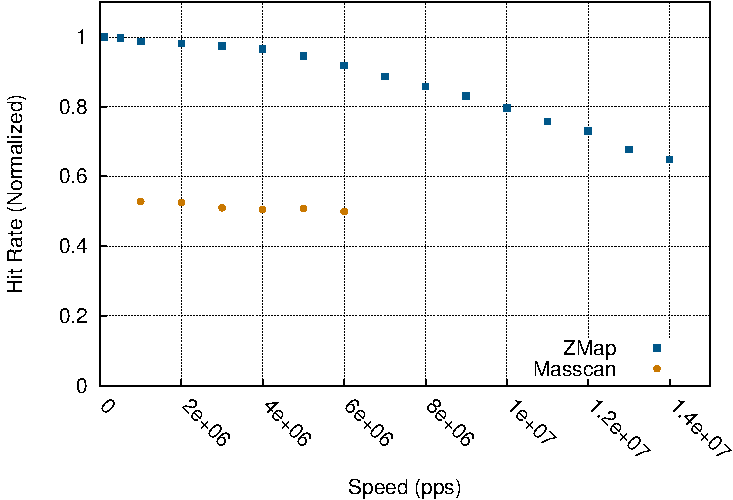
\includegraphics[height=2.1in]{\ZippyFigures/norm_avg_hitrate.pdf}
\caption{\textbf{Hit-rate vs.\ Scan-rate}\,---\,%
ZMap's hit rate is roughly stable up to a scan rate of 4~Mpps, then declines
linearly. This drop off may be due to upstreudegrm network congestion. Even using
PF\_RING, Masscan is unable to achieve scan rates above 6.4~Mpps on the same
hardware and has a much lower hit rate.}
\label{fig:hitrate}
\end{figure}

\begin{figure}[t]\centering
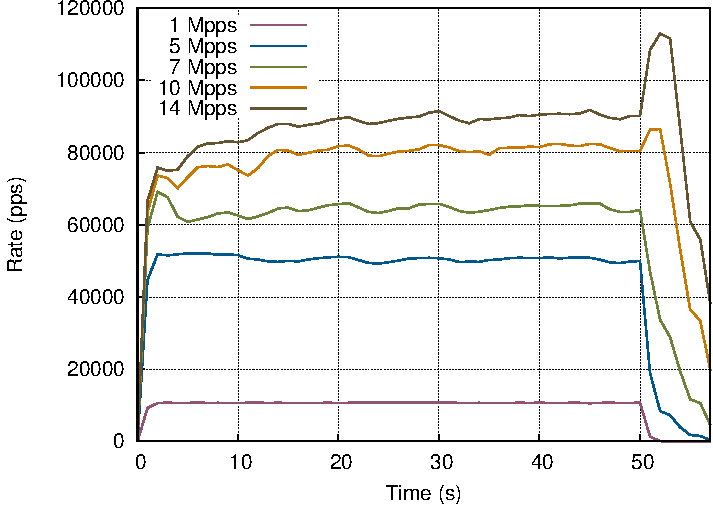
\includegraphics[height=2.1in]{\ZippyFigures/avg_count_recv_succs.pdf}
\caption{\textbf{Response Rate During Scans}\,---\,%
This graph shows the rate of incoming SYN-ACKs during 50-second scans. The
peaks at the end (after sending finishes) at rates above 7~Mpps indicate that
many responses are being dropped and retransmitted before being recorded by
ZMap.}
\label{fig:recvrate}
\end{figure}

We first investigate whether response packets are being dropped by ZMap or
the network. In the original ZMap work, we found that 99\% of hosts respond
within 1~second~\cite{zmap}. As such, we would expect that after 1~second,
there would be negligible responses. However, as can be seen in
Figure~\ref{fig:recvrate}, there is an unexpected spike in response packets
after sending completes at 50~seconds for scans at 10 and 14~Mpps. This spike
likely indicates that response packets are being dropped by our network, NIC,
or ZMap, as destination hosts will resend SYN-ACK packets for more than one
minute if an ACK or RST packet is not received.

In order to determine whether the drop of response packets is due to ZMap
inefficiencies or upstream network congestion, we performed a secondary scan
in which we split the probe generation and address processing onto separate
machines. The send machine remained the same. The receive machine was an HP
ProLiant DL120 G7, with an Intel Xeon E3-1230 processor (4 cores with
hyperthreading) and 16~GB of memory, running Ubuntu 12.04.4~LTS and the
3.5.0-52-generic Linux kernel.

As we show in Figure~\ref{fig:twomachines}, this spike does not occur when
processing response packets on a secondary server---instead it closely
follows the pattern of the slower scans. This indicates that ZMap is locally
dropping response packets. However, the split setup received only 4.3\% more
packets than the single machine---not enough to account for the 31.7\%
difference between a 14~Mpps and a 1~Mpps scan. If a large number of response
packets were dropped due to network congestion, we would not have observed an
immediate drop in responses---likely indicating that the root cause of the
decreased hit-rate is dropped probe packets.

It is not immediately clear where probe packets are dropped---it is possible
that packets are dropped locally by PF\_RING, are dropped by local routers
due to congestion, or that we are overwhelming destination networks. PF\_RING
records locally dropped packets, which remained zero throughout our scans,
which indicates that packets are not being dropped locally. In order to
locate where packet drop is occurring on our network, we calculated the drop
rate per AS and found little AS-level correlation for packets dropped by the
10\,GigE scans, which suggests that random packet drop is occurring close to
our network rather than at particular distant destination networks.

\begin{figure}\centering
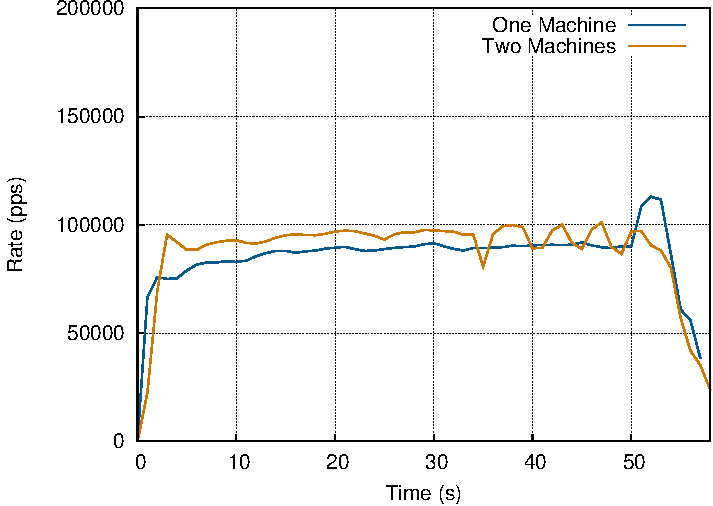
\includegraphics[width=\linewidth]{\ZippyFigures/split_avg_count_recv_succs.pdf}
\caption{\textbf{Comparing One and Two Machines}\,---\,%
If we scan at 14~Mpps and use separate machines for the sending and receiving
tasks, the spike in the SYN-ACK rate at 50~s disappears, indicating that
fewer packets are dropped with the workload spread over two machines.
However, overall the two machine configuration received only 4.3\% more
responses than with one machine, which suggests that network packet loss
accounts for the majority of the drop off at higher scan rates.}
\label{fig:twomachines}
\end{figure}

\subsection{Complete Scans}

We completed a full Internet-wide scan, allowing ZMap to operate at its full
scan rate. This scan achieved an average 14.23~Mpps---96\% of the theoretical
limit of 10\,GigE, completing in 4~minutes, 29~seconds and achieving a hit
rate that is 62.5\% of that from a 1\,GigE scan. We show a comparison to
lower speed scans in Table~\ref{tbl:fullhitrate}. As we discussed in the
previous section, this decrease is likely due to local network congestion,
which results in dropped probe packets. However, more investigation is
deserved in order to understand the full dynamics of high-speed scans.

\subsection{Comparison to Masscan}
\label{sec:masscan-comparison}

\begin{figure*}\centering
\hfill
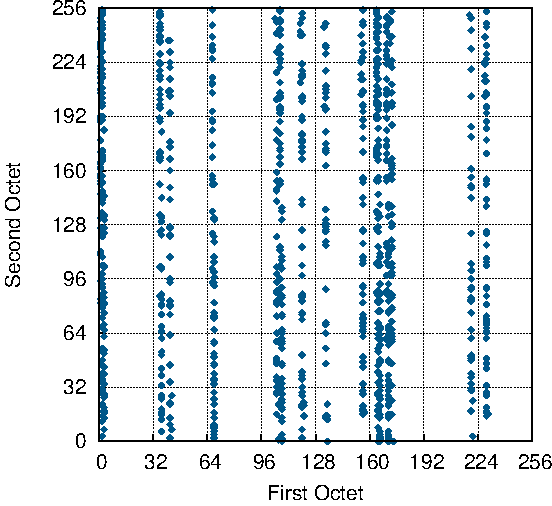
\includegraphics[height=2.5in]{\ZippyFigures/masscan_randomness.pdf}
\hfill\hfill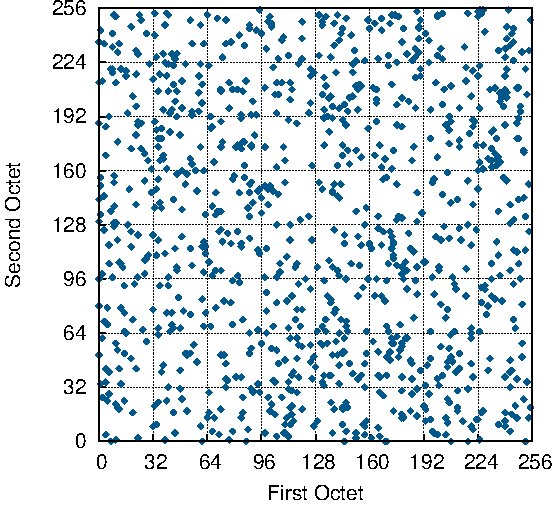
\includegraphics[height=2.5in]{\ZippyFigures/zmap_randomness.pdf}
\hfill\strut
\caption{\textbf{Address Randomization Comparison}\,---\,%
These plots depict the first 1000 addresses of an Internet-wide scan selected
by Masscan (\emph{left}) and ZMap (\emph{right}), with the first and second
octets mapped to the $x$ and~$y$ coordinates. ZMap's address randomization is
CPU intensive but achieves better statistical properties than the cheaper
approach used by Masscan, enabling valid sampling. We enhanced ZMap to
distribute address generation across multiple cores.}
\label{fig:randomy}
\end{figure*}

Masscan advertises the ability to emit probes at 25~Mpps using PF\_RING and
two 10\,GigE adapters, each configured with two RSS queues---84\% of
linespeed for dual 10\,GigE and 166\% of linespeed for a single 10\,GigE
adapter~\cite{masscan-10g}. We benchmarked ZMap and Masscan using the
Xeon~E3-1230 machine described above. In our experiments, we found that
Masscan was able to send at a peak 7.4~Mpps using a single-adapter
configuration with two RSS queues, 50\% of 10\,GigE linespeed. On the same
hardware, ZMap is capable of reaching a peak 14.1~Mpps. While Masscan may be
able to achieve a higher maximum speed using multiple adapters, ZMap is able
to fully saturate a 10\,GigE uplink with a single adapter.

Masscan uses a custom Feistel network to ``encrypt'' a monotonically
increasing index to generate a random permutation of the IPv4 address
space~\cite{masscan-rng}. While this is computation cheaper than using a
cyclic group, this technique results in poor statistical properties, which we
show in Figure~\ref{fig:randomy}. This has two consequences: first, it is not
suitable for sampling portions of the address space, and second, there is
greater potential for overloading destination networks. This could explain
the discrepency in Figure~\ref{fig:hitrate} if Masscan targeted a less
populated subnet.

Masscan and ZMap use a similar sharding approach to parallelize address
generation and distribute scans. Both programs ``count off'' addresses into
shards by staggering the offsets of the starting position of each shard
within the permutation and iterating a fixed number of steps through each of
their permutations. In ZMap, this is implemented by replacing the iteration
factor $g$ with $g^n$. In Masscan, this is simply a matter of incrementing
the monotonically increasing index by more than one.


\section{Applications}
\label{sec:discussion}

In this section, we consider applications that could benefit from 10\,GigE
scanning and remark on the implications of high-speed scanning for defenders
and attackers.

Scanning at faster rates reduces the blur introduced from hosts changing IP
addresses by decreasing the number of hosts that may be doubly counted during
longer scans. This also increases the ability to discover hosts that are only
online briefly. Thus, the ability to complete scans in minutes allows
researchers to more accurately create a snapshot of the Internet at a given
moment.

Similarly, the increased scan rate enables researchers to complete
high-resolution scans when measuring temporal effects. For example, while
researchers were able to complete comprehensive scans for the recent
Heartbleed Vulnerability every few hours~\cite{zmap-heartbleed}, many sites
were patched within the first minutes after disclosure. The ability to scan
more rapidly could help shed light on patching behavior within this critical
initial period.

\begin{figure*}
\centering
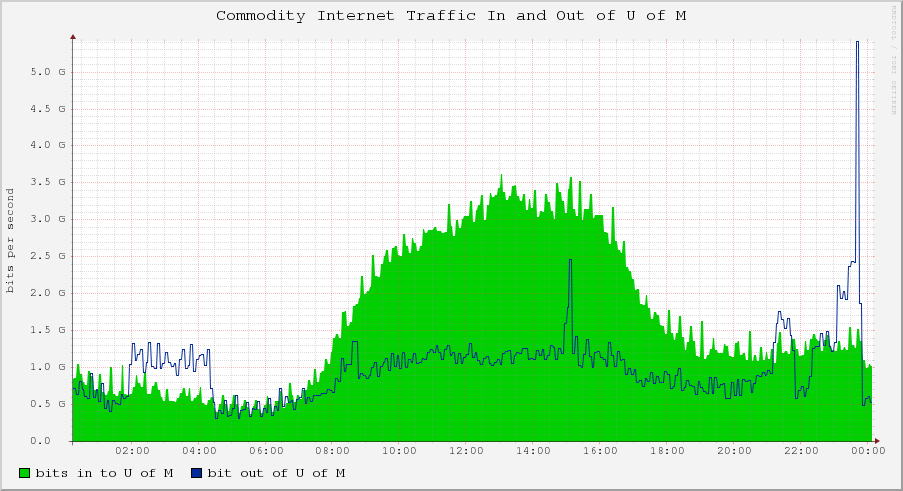
\includegraphics[width=0.75\linewidth]{\ZippyFigures/graph_image.png}
\caption{\textbf{10\,GigE   Scan Traffic}\,---\,%
An Internet-wide scan at full 10\,GigE speed dwarfed all other traffic at the
university during this 24~hour period. At 14.23~Mpps, a single machine
running ZMap generated 4.6~Gbps in outgoing IP traffic and scanned the entire
public IPv4 address space in 4m29s. The massive increase in outbound traffic
appears to have caused elevated packet drop. Notable smaller spikes are due
to earlier experiments.}
\label{fig:traffic}
\end{figure*}

Faster scan rates also allow for a variety of new scanning-related
applications that require multiple packets, including quickly completing
global trace routes or performing operating system fingerprinting.
Furthermore, the advancement of single-port scanning can be utilized to
quickly perform scans of a large number of ports, allowing scanning all
privileged ports on a /16 in under 5~seconds and \emph{all} ports in
5~minutes, assuming the attacker has sufficient bandwidth to the target.

The most alarming malicious potential for 10\,GigE scanning lies in its
ability to find and exploit vulnerabilities \emph{en masse} in a very short
time. Durumeric et~al.\ found that attackers began scanning for the
Heartbleed vulnerability within 22~hours of its
disclosure~\cite{zmap-heartbleed}. While attackers have utilized botnets and
worms in order to complete distributed scans for vulnerabilities, recent
work~\cite{state-of-scanning} has shown that attackers are now also using
ZMap, Masscan, and other scanning technology from bullet-proof hosting
providers in order to find vulnerable hosts. The increase in scan rates could
allow attackers to complete Internet-wide vulnerability scans in minutes as
10\,GigE becomes widely available.\looseness=-1

\section{Future Work}

We demonstrated that it is possible to perform Internet-wide scans at
10\,GigE linespeed, but, at least from our institutional network, we are
unable to sustain the expected hit rate as scanning approaches this packet
rate. Further investigation is needed to understand this effect and profile
ZMap's performance on other networks. One important question is whether the
drop off is caused by nearby network bottlenecks (which might be reduced with
upgraded network hardware) or whether it arises because such rapid scanning
induces congestion on many distant networks---which would represent an
inherent limit on scan speed. It is also possible that there are a small
number of remote bottlenecks that cause the observed drop in hit rate at high
speeds. In that case, identifying, profiling, and removing these bottlenecks
could improve performance.

40\,GigE hardware currently exists, and 100\,GigE is under
development~\cite{hundred-gig}. As these networks become more widely
available, it may be desirable to optimize and scale Internet-wide scanning
to even higher speeds.

\section{Conclusion}

In this work, we introduced enhancements to the ZMap Internet scanner that
enable it to scan at up to 14.2~Mpps. The three modifications we
present---sharding, optimized address constraints, and integration with
PF\_RING ZC---enable scanning at close to 10\,GigE linespeed. These
modifications are available now on experimental ZMap branches and will be
merged into mainline ZMap.

With these enhancements, we are able to complete a scan of the public IPv4
address space in 4m29s. However, despite having a well provisioned upstream
network, coverage in our experiments drops precipitously when scanning faster
than 4~Mpps. While further research is needed to better characterize and
reduce the causes of this drop off, it may be related to specific conditions
on our network.

As faster network infrastructure becomes more widely available, 10\,GigE
scanning will enable powerful new applications for both researchers and
attackers.

\section*{Acknowledgments}

The authors thank the exceptional sysadmins at the University of Michigan for
their help and support throughout this project. This research would not have
been possible without Kevin Cheek, Chris Brenner, Laura Fink, Paul Howell,
Don Winsor, and others from ITS, CAEN, and DCO\@. We are grateful to Michael
Bailey for numerous productive discussions, to Luca Deri and ntop for
providing a PF\_RING license, and to the many contributors to the ZMap open
source project. We also thank Denis Bueno, Jakub Czyz, Henry Fanson, Pat
Pannuto, and Eric Wustrow.

This material is based upon work supported by the National Science Foundation
under Grant No.~CNS-1255153 and No.~CNS-0964545. Any opinions, findings, and
conclusions or recommendations expressed in this material are those of the
authors and do not necessarily reflect the views of the National Science
Foundation.

%% !TEX root = ../../../proposal.tex

{\footnotesize\bibliographystyle{abbrv}
\balance
\bibliography{woot}}
\end{document}




\chapter{Conclusion and Future Work}

Concluding thoughts.

Future work

\section{Future Idea A}
Graduate.

\section{Future Idea B}
Startup.

\section{Shaping security behavior}
Cash money.

\bibliographystyle{plain}
\bibliography{refs}

\end{document}
